\documentclass[%
   final,      % fertiges Dokument
%%%% --- Schriftgröße ---
   11pt, 
   headings=big,
%%%% --- Sprache ---
   ngerman,           % wird an andere Pakete weitergereicht
%%%% === Seitengröße ===
   a4paper,
%%%% === Optionen für den Satzspiegel ===
   BCOR=5mm,          % Zusaetzlicher Rand auf der Innenseite
   DIV=11,           % Seitengroesse (siehe Koma Skript Dokumentation !)
   1.1headlines,     % Zeilenanzahl der Kopfzeilen
   headinclude=false,   % Kopf nicht einbeziehen
   footinclude=false,   % Fuss nicht einbeziehen
   mpinclude=false,     % Margin nicht einbeziehen
   pagesize,         % Schreibt die Papiergroesse in die Datei.
                     % Wichtig fuer Konvertierungen
%%%% === Layout ===
   %oneside,       % einseitiges Layout  
   %twoside,
    openany,  % Kapitel beginnen auf jeder Seite
   titlepage,        % Titel als einzelne Seite ('titlepage' Umgebung)
%%%% --- Absatzeinzug ---
   parskip=false,        % Eingerückt (Standard)
%%%% --- Kapitel ---
   chapterprefix=false,  % keine Ausgabe von 'Kapitel:'
%%%% === Verzeichnisse (TOC, LOF, LOT, BIB) ===
   bibliography=totoc,         % Bibliographie ins TOC
   toc=graduated,        % eingereuckte Gliederung
   listof=graduated,      % eingereuckte LOT, LOF
   numbers=enddot,  % Überschriftnummerierung mit Punkt, siehe DUDEN !
]{scrbook}

%%%%%%%%%%%%%%%%%%%%%%%%%%%%%%%%%%%%%%%%%%%%%%%%%%%%%%%
% Preambel
% preamble
%%%%%%%%%%%%%%%%%%%%%%%%%%%%%%%%%%%%%%%%%%%%%%%%%%%%%%%%%%%%%%%%%%%%%%%%%%%%%%%%%%%%
%  Allgemein
%\usepackage[latin1]{inputenc}
\usepackage[ngerman]{babel}     % Deutsche Sprache in automatmisch generiertem
\usepackage[utf8]{inputenc}     %  =E4 =F6 =FC =DF; danach  geht auch das ß richtig
\usepackage{longtable}
\usepackage{latexsym}           % Fuer recht seltene Zeichen
\usepackage{caption}            % Figure-Captions formatieren
\usepackage{sectsty}            % Section headings formatieren   
\usepackage{xparse}             % Für selbstgeschrieben Befehle 
\usepackage{lmodern}
 
%%%%%%%%%%%%%%%%%%%%%%%%%%%%%%%%%%%%%%%%%%%%%%%%%%%%%%%%%%%%%%%%%%%%%%%%%%%%%%%%%%%%
%%%%%%  Layout
	\usepackage[left=3cm,right=2.5cm,top=2.2cm,bottom=2.2cm,includeheadfoot]{geometry}

	%%%%%% Fonts
	\usepackage[T1]{fontenc} % T1 Schrift Encoding
	\usepackage{lmodern}
	%\usepackage[table]{xcolor}
	\usepackage[normalem]{ulem}	% unterstreichen im Text

	\usepackage[ngerman]{varioref} % Intelligente Querverweise

	%%%%%% Kopf und Fusszeile
	\usepackage[%
	   automark,         % automatische Aktualisierung der Kolumnentitel
	   markcase=ignoreuppercase,      % Grossbuchstaben verhindern
	]{scrlayer-scrpage}

	\pagestyle{scrheadings}
	% loescht voreingestellte Stile
	\clearscrheadings
	\clearscrplain
	% Was steht wo...
	   \ohead{\pagemark}
	   \ihead{\headmark}
	   \ofoot[\pagemark]{} % Außen unten: Seitenzahlen bei plain

	% Angezeigte Abschnitte im Header
	   \automark[section]{chapter} %[rechts]{links}
	%
	% Linien (moegliche Kombination mit Breiten)
	\setheadsepline{.4pt}[\color{black}]

	\setheadwidth[0pt]{text}
	\setfootwidth[0pt]{text}

%%%%%%%%%%%%%%%%%%%%%%%%%%%%%%%%%%%%%%%%%%%%%%%%%%%%%%%%%%%%%%%%%%%%%%%%%%%%%%%%%%%%
%  Bib und Links
	\usepackage[%
		square,	% for square brackets;
		comma,	% to use commas as separaters;
		numbers,	% for numerical citations;
		sort,		% orders multiple citations into the sequence in which they appear in the list of references;
		sort&compress,    % as sort but in addition multiple numerical citations
					   % are compressed if possible (as 3-6, 15);
	]{natbib}
	\bibliographystyle{dinat}

    \usepackage[margin=0pt]{subcaption} % specific form for captions
    \usepackage[autostyle]{csquotes} % helper for quoting


	\usepackage[
	   % Farben fuer die Links
	   colorlinks=true,         % Links erhalten Farben statt Kaeten
	   urlcolor=true,    % \href{...}{...} external (URL)
	   filecolor=true,  % \href{...} local file
	   linkcolor=true,  %\ref{...} and \pageref{...}
	   % Links
	   raiselinks=true,			 % calculate real height of the link
	   breaklinks,              % Links berstehen Zeilenumbruch
	   backref=page,            % Backlinks im Literaturverzeichnis (section, slide, page, none)
	   pagebackref=false,        % Backlinks im Literaturverzeichnis mit Seitenangabe
	   verbose,
	   hyperindex=true,         % backlinkex index
	   linktocpage=true,        % Inhaltsverzeichnis verlinkt Seiten
	   hyperfootnotes=false,     % Keine Links auf Fussnoten
	   % Bookmarks
	   bookmarks=true,          % Erzeugung von Bookmarks fuer PDF-Viewer
	   bookmarksopenlevel=1,    % Gliederungstiefe der Bookmarks
	   bookmarksopen=true,      % Expandierte Untermenues in Bookmarks
	   bookmarksnumbered=true,  % Nummerierung der Bookmarks
	   bookmarkstype=toc,       % Art der Verzeichnisses
	   % Anchors
	   plainpages=false,        % Anchors even on plain pages ?
	   pageanchor=true,         % Pages are linkable
	   % PDF Informationen
	   pdfpagelabels=true,      % set PDF page labels
	]{hyperref}
	
%%%%%%%%%%%%%%%%%%%%%%%%%%%%%%%%%%%%%%%%%%%%%%%%%%%%%%%%%%%%%%%%%%%%%%%%%%%%%%%%%%%%
%  Mathekram
	\usepackage{,amsfonts,amssymb,amsthm} % mathematical expression, symbols, fonts, and the whole theorem environment engine
	\usepackage[
	   intlimits,  % Like sumlimits, but for integral symbols.
		]{amsmath}	% math package with additional symbols
	\usepackage{icomma}			% Erlaubt die Benutzung von Kommas im Mathematikmodus
	\usepackage{units}				% for units
	\usepackage{caption}			
	\usepackage{pdfpages}			% include whole pdf files
	\usepackage{ragged2e}			% Besserer Flatternsatz (Linksbuendig, statt Blocksatz)
% Nützliche Abkürzungen
    \newcommand{\NN}{\mathbb{N}} % natürliche Zahlen
    \newcommand{\RR}{\mathbb{R}} % reelle Zahlen
    \newcommand{\QQ}{\mathbb{Q}} % rationale Zahlen
    \newcommand{\ZZ}{\mathbb{Z}} % ganze Zahlen
%%%%%%%%%%%%%%%%%%%%%%%%%%%%%%%%%%%%%%%%%%%%%%%%%%%%%%%%%%%%%%%%%%%%%%%%%%%%%%%%%%%%
%  Bilder
	\usepackage{tikz}
    \usepackage{siunitx}
    \usepackage{standalone}
 	\usetikzlibrary{positioning, calc,quotes,angles,arrows,decorations.pathmorphing,decorations.pathreplacing,quotes} 
    \usetikzlibrary{shapes,backgrounds,fit,matrix}
    \usepackage{svg}                % für das einbinden von svg bildern
	\usepackage{float}              % Stellt die Option [H] fuer Floats zur Verfgung
   
	\usepackage[figure]{hypcap}     % Links auf Gleitumgebungen springen nicht zur Beschriftung,
	                                % sondern zum Anfang der Gleitumgebung
%    \usepackage{xcolor,graphicx}    % graphics and colorings
  
  \usepackage{graphicx}           %zusätzlich zu wrapfig zum einfügen von bildern der benötigt wird. 
    \usepackage{wrapfig}            %Textumflossene Bilder die nicht Textblock-Breite sind 
    

%%%%%%%%%%%%%%%%%%%%%%%%%%%%%%%%%%%%%%%%%%%%%%%%%%%%%%%%%%%%%%%%%%%%%%%%%%%%%%%%%%%%
%  Tabellen
	\usepackage{tabularx}		% Automatische Spaltenbreite
	\usepackage{booktabs} 		% bessere Abstaende innerhalb der Tabelle (Layout))
	\usepackage{multirow}       % Mehrfachspalten
    \usepackage{rotating}       % if you want to rotate any object
%%%%%%%%%%%%%%%%%%%%%%%%%%%%%%%%%%%%%%%%%%%%%%%%%%%%%%%%%%%%%%%%%%%%%%%%%%%%%%%%%%%%%
%  Pseudocode
\usepackage[ruled,vlined,linesnumbered,german,onelanguage]{algorithm2e}
\usepackage{algpseudocode}

%%%%%%%%%%%%%%%%%%%%%%%%%%%%%%%%%%%%%%%%%%%%%%%%%%%%%%%%%%%%%%%%%%%%%%%%%%%%%%%%%%%%%
% theorem und beweise

%\cref is a powerfull command that automatically states the current environment (e.g. Theorem, Lemma, etc.)
\usepackage[sort&compress,nameinlink,noabbrev,capitalize]{cleveref}
\usepackage{scrextend} % super powerful tool that helps a bit with everything





%DIF PREAMBLE EXTENSION ADDED BY LATEXDIFF
%DIF UNDERLINE PREAMBLE %DIF PREAMBLE
\RequirePackage[normalem]{ulem} %DIF PREAMBLE
\RequirePackage{color}\definecolor{RED}{rgb}{1,0,0}\definecolor{BLUE}{rgb}{0,0,1} %DIF PREAMBLE
\providecommand{\DIFadd}[1]{{\protect\color{blue}\uwave{#1}}} %DIF PREAMBLE
\providecommand{\DIFdel}[1]{{\protect\color{red}\sout{#1}}}                      %DIF PREAMBLE
%DIF SAFE PREAMBLE %DIF PREAMBLE
\providecommand{\DIFaddbegin}{} %DIF PREAMBLE
\providecommand{\DIFaddend}{} %DIF PREAMBLE
\providecommand{\DIFdelbegin}{} %DIF PREAMBLE
\providecommand{\DIFdelend}{} %DIF PREAMBLE
\providecommand{\DIFmodbegin}{} %DIF PREAMBLE
\providecommand{\DIFmodend}{} %DIF PREAMBLE
%DIF FLOATSAFE PREAMBLE %DIF PREAMBLE
\providecommand{\DIFaddFL}[1]{\DIFadd{#1}} %DIF PREAMBLE
\providecommand{\DIFdelFL}[1]{\DIFdel{#1}} %DIF PREAMBLE
\providecommand{\DIFaddbeginFL}{} %DIF PREAMBLE
\providecommand{\DIFaddendFL}{} %DIF PREAMBLE
\providecommand{\DIFdelbeginFL}{} %DIF PREAMBLE
\providecommand{\DIFdelendFL}{} %DIF PREAMBLE
%DIF LISTINGS PREAMBLE %DIF PREAMBLE
\RequirePackage{listings} %DIF PREAMBLE
\RequirePackage{color} %DIF PREAMBLE
\lstdefinelanguage{DIFcode}{ %DIF PREAMBLE
%DIF DIFCODE_UNDERLINE %DIF PREAMBLE
  moredelim=[il][\color{red}\sout]{\%DIF\ <\ }, %DIF PREAMBLE
  moredelim=[il][\color{blue}\uwave]{\%DIF\ >\ } %DIF PREAMBLE
} %DIF PREAMBLE
\lstdefinestyle{DIFverbatimstyle}{ %DIF PREAMBLE
	language=DIFcode, %DIF PREAMBLE
	basicstyle=\ttfamily, %DIF PREAMBLE
	columns=fullflexible, %DIF PREAMBLE
	keepspaces=true %DIF PREAMBLE
} %DIF PREAMBLE
\lstnewenvironment{DIFverbatim}{\lstset{style=DIFverbatimstyle}}{} %DIF PREAMBLE
\lstnewenvironment{DIFverbatim*}{\lstset{style=DIFverbatimstyle,showspaces=true}}{} %DIF PREAMBLE
%DIF END PREAMBLE EXTENSION ADDED BY LATEXDIFF







% commands
%%%%%%%%%%%%%%%%%%%%%%%%%%%%%%%%%%%%%%%%%%%%%%%%%%%%%%%%%%%%%%%%%%%%%%%%%%%%%%%%%%%%
% Einrückung global entfernen
\setlength{\parindent}{0pt}

%%%%%%%%%%%%%%%%%%%%%%%%%%%%%%%%%%%%%%%%%%%%%%%%%%%%%%%%%%%%%%%%%%%%%%%%%%%%%%%%%%%%
% maximal zulässigen Wortabstand einstellen
\setlength\emergencystretch{1em} 

%%%%%%%%%%%%%%%%%%%%%%%%%%%%%%%%%%%%%%%%%%%%%%%%%%%%%%%%%%%%%%%%%%%%%%%%%%%%%%%%%%%%
% Farben fuer Verlinkungen definieren/aendern
 \usepackage{color}
   %Linkfarbe setzen
   \definecolor{LinkColor}{gray}{0}
   %PDF Farben einstellen
   \hypersetup{colorlinks=true,%
   linkcolor=LinkColor,%
   citecolor=LinkColor,%
   filecolor=LinkColor,%
   menucolor=LinkColor,%
   urlcolor=LinkColor} 
   
%%%%%%%%%%%%%%%%%%%%%%%%%%%%%%%%%%%%%%%%%%%%%%%%%%%%%%%%%%%%%%%%%%%%%%%%%%%%%%%%%%%%
% Aussehen der Ueberschriften

	\setkomafont{chapter}{\huge\sffamily}    % Chapter
	\setkomafont{sectioning}{\sffamily} %  % Titelzeilen % \bfseries
	\setkomafont{pagenumber}{\sffamily}             % Seitenzahl
	\setkomafont{descriptionlabel}{\itshape}        % Kopfzeile
	%
	\addtokomafont{sectioning}{\color{black}} % Farbe der Ueberschriften
	\addtokomafont{chapter}{\color{black}} % Farbe der Ueberschriften
	\renewcommand*{\raggedsection}{\raggedright} % Titelzeile linksbuendig, haengend

%%%%%%%%%%%%%%%%%%%%%%%%%%%%%%%%%%%%%%%%%%%%%%%%%%%%%%%%%%%%%%%%%%%%%%%%%%%%%%%%%%%%
% Silbentrennung
	\hyphenation{}
	
%%%%%%%%%%%%%%%%%%%%%%%%%%%%%%%%%%%%%%%%%%%%%%%%%%%%%%%%%%%%%%%%%%%%%%%%%%%%%%%%%%%%
% Feste Spaltenbreiten zentriert, linksbuendig oder rechtsbuendig	
\newcolumntype{L}[1]{>{\raggedright\arraybackslash}p{#1}} % linksbündig mit Breitenangabe
\newcolumntype{C}[1]{>{\centering\arraybackslash}p{#1}} % zentriert mit Breitenangabe
\newcolumntype{R}[1]{>{\raggedleft\arraybackslash}p{#1}} % rechtsbündig mit Breitenangabe	


% theorem environment
\theoremstyle{plain} % typical theorem-style (bold header, italic font)
\newtheorem{theorem}{Theorem}[section]
\newtheorem{lemma}[theorem]{Lemma}
\newtheorem{corollary}[theorem]{Korollar}
\newtheorem{observation}[theorem]{Beobachtung}
\newtheorem{proposition}[theorem]{Proposition}
\newtheorem{rrule}{Reduktionsregel}[section]

\crefname{rrule}{Reduktionsregel}{Reduktionsregeln} % how cleverref (\cref) has to handle these environments
\Crefname{rrule}{RR}{RRs} % with \Cref us can use what you defined here---somtimes useful if you want to abbreviate environment when citing (e.g. in tables or figures)

\theoremstyle{definition} % typical definition-style (bold header, normal font)
\newtheorem{definition}[theorem]{Definition}

\theoremstyle{remark} % typical theorem-style (italic header, normal font)
\newtheorem{example}{Example}
\newtheorem*{remark}{Remark}
\newtheorem{reduction}{Reduction}
\theoremstyle{plain}

% problem definition evironment: gets three arguments (1) problem name #1 (2) input specification #2 (3) question specification #3
\newcommand{\problemdef}[3]{
  \begin{center}
    \begin{minipage}{0.95\textwidth}
      \noindent
      \textsc{#1}
      
      \vspace{2pt}
      \setlength{\tabcolsep}{3pt}
      \begin{tabularx}{\textwidth}{@{}lX@{}}
        \textbf{Eingabe:} 		& #2 \\
        \textbf{Frage:} 	& #3
      \end{tabularx}
    \end{minipage}
  \end{center}
}



	
%%%%%%%%%%%%%%%%%%%%%%%%%%%%%%%%%%%%%%%%%%%%%%%%%%%%%%%%%%%%%%%%%%%%%%%%%%%%%%%%%%%%
% Macros 

% \NewDocumentCommand{\foocmd}{ O{default1} O{default2} m }{#1 #2 #3}
%                         %     ⤷ #1        ⤷ #2    ⤷ #3

%   \foocmd{foo} \par                           default1 default2 foo
%   \foocmd[nondefault1]{foo} \par              nondefault1 default2 foo
%   \foocmd[nondefault2][notfoo2]{foo} \par     nondefault12 notfoo2 foo


\newboolean{boolvar} %Deklaration
\setboolean{boolvar}{true} %Zuweisung

 \NewDocumentCommand{\todo}{  O{ueberarbeiten!} O{red}  }{
 \ifthenelse{\boolean{boolvar}}
    { [\textcolor{#2}{TODO: #1 }]  }
    { %[\textcolor{$2}{TODO: $1 }]  }

    }
} 

% \newcommand{\delaunayRefinement}{Delaunay-Refinement }
% \newcommand{\delaunayRefinements}{Delaunay-Refinements }
% \newcommand{\delaunayTriagnulierung}{Delaunay-Triagnulierung}

 
 \NewDocumentCommand{\innenwinkel}{ s O{i} O{j} O{k}  }{
 \IfBooleanTF #1 
 {\theta_{#2}^{#3,#4}}
 {$\theta_{#2}^{#3,#4}$} 
 }
 \NewDocumentCommand{\nominnenwinkel}{ s O{i} O{j} O{k}  }{
 \IfBooleanTF #1 
 {\tilde{\theta}_{#2}^{#3,#4}} 
 {$\tilde{\theta} _{#2}^{#3,#4}$}
 }
 
 \NewDocumentCommand{\gesamtwinkel}{s O{i}}{
   \IfBooleanTF #1 
 {\Theta_{#2}}
 {$\Theta_{#2}$} 
 }
 
 \NewDocumentCommand{\bezugsrichtung}{s O{i}}{
   \IfBooleanTF #1 
 {e_{#2}}
 {$e_{#2}$}
 }
 
  \NewDocumentCommand{\richtung}{s O{i}}{
   \IfBooleanTF #1 
 {\phi_{#2}}
 {$\phi_{#2}$}
 }
 
 
 
 \NewDocumentCommand{\algorithmusname}{s O{i}}{
   \IfBooleanTF #1 
 {\text{intrinsisches Delaunay-Refinement}}
 {intrinsisches Delaunay-Refinement}
 }
 
 
 %umkreisradius-kürzeste-kante-verhältnis 
 \NewDocumentCommand{\kuezesteKante}{s}{
    \IfBooleanTF #1 
        {l}
        {$l$}
 }
 \NewDocumentCommand{\umkreisradius}{s}{
     \IfBooleanTF #1 
        {r}
        {$r$}
 }
  \NewDocumentCommand{\kleinsterWinkel}{s}{
     \IfBooleanTF #1 
        {\Theta_{\text{min}}}
        {$\Theta_{\text{min}}$}
 }
 
   \NewDocumentCommand{\Dichte}{s O{v}}{
     \IfBooleanTF #1 
        {D_{#2}}
        {$D_{#2}$}
 }
 
 
    \NewDocumentCommand{\irregulaereKante}{s O{(v,v)}}{
     \IfBooleanTF #1 
        {e_{#2}}
        {$e_{#2}$}
 }
 
 
    \NewDocumentCommand{\regulaereKante}{s O{(v,s)}}{
     \IfBooleanTF #1 
        {e_{#2}}
        {$e_{#2}$}
 }
 
 \NewDocumentCommand{\UrzkK}{s O{(v,s)}}{
          \IfBooleanTF #1 
        {\kappa}
        {$\kappa$}
 }

 
 
 
 
 
 
 
 


\begin{document}
%%%%%%%%%%%%%%%%%%%%%%%%%%%%%%%%%%%%%%%%%%%%%%%%%%%%%%%
% Deckblatt
	
% %%%%%%%%%%%%%%%%%%%%%%%%%%%%%%%%%%%%%%%%%%%%%%%%%%%%%%%
% Verzeichnisse und Co
	\frontmatter
	    \begin{titlepage}
	\sffamily
    \raggedleft
	\small
	\begin{center}		
		\color{gray}
		\begin{tabularx}{\textwidth}{R{0.5\textwidth}L{0.5\textwidth}}
			
\includegraphics[width=0.25\textwidth]{images/Logo_TU.pdf}&\\
			&\textbf{Fakultät IV}\\
			&\textbf{Elektrotechnik und Informatik}\\
			&\textbf{Institut für Technische Informatik und Mikroelektronik}\\
			&\textbf{Fachgebiet Computer Graphics}\\
			&\textbf{Prof. Dr. Marc Alexa}\\
		\end{tabularx}	
	\end{center}
	\mbox{}\vspace{2\baselineskip}\\
	\sffamily\huge
	\centering   
	%TODO Bachlorarbeit größer
	Bachelorarbeit:\vspace{0.25\baselineskip}\\
	%\vspace{2\baselineskip}\\
	\sffamily\Huge
Winkeldefektbedingungen für intrinsisches \delaunayRefinement \vspace{1.5\baselineskip}\\
	\sffamily\normalsize
	Vorgelegt von:\vspace{0.5\baselineskip}\\	
	Tarik Abdel-Moati Moussa Salama\vspace{0.25\baselineskip}\\
	Matrikelnummer 380833\vspace{0.25\baselineskip}\\
	
	\sffamily\large
	Berlin, den \today
	\vspace{3\baselineskip}\\

   \vfill
   \raggedright
   \small 
   \centering
	\vfill	
	\uline{Erstgutachter:}\vspace{0.25\baselineskip}\\
	Prof. Dr. Marc Alexa (TU Berlin)\vspace{0.5\baselineskip}\\
	\uline{Zweitgutachter:}\vspace{0.25\baselineskip}\\
	Prof. Dr. Alexander I. Bobenko (TU Berlin)
	\vspace{2\baselineskip}\\
	\uline{Betreuer:}\vspace{0.25\baselineskip}\\
	Ugo Paavo Finnendahl (TU Berlin)\vspace{0.25\baselineskip}\\
	%Carl Lutz (TU Berlin)\\

\end{titlepage}

	    \cleardoublepage
		% Die eidesstattliche Erklärung mit Unterschrift
\chapter*{Erklärung der Urheberschaft}
Hiermit erkläre ich an Eides statt gegenüber der Fakultät I der Technischen Universität Berlin, dass die 
vorliegende, dieser Erklärung angefügte Arbeit  selbstständig und nur unter Zuhilfenahme der im 
Literaturverzeichnis genannten Quellen und Hilfsmittel angefertigt wurde. Alle Stellen der Arbeit, die anderen 
Werken dem Wortlaut oder dem Sinn nach entnommen wurden, sind kenntlich gemacht. Ich reiche die Arbeit 
erstmals als Prüfungsleistung ein. Ich versichere, dass diese Arbeit oder wesentliche Teile dieser Arbeit 
nicht bereits dem Leistungserwerb in einer anderen Lehrveranstaltung zugrunde lagen.

\vspace{4cm}



%\hrulefill
\noindent
%\hspace{2cm}
Berlin, den \today %\hfill 
\makebox[0pt][l]{\hspace*{2cm}\raisebox{-5ex}{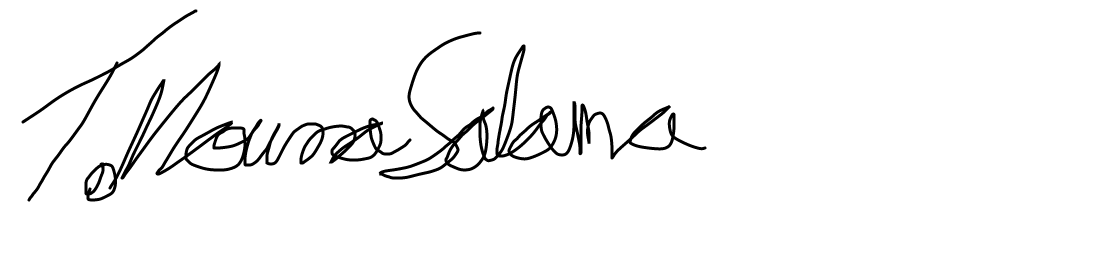
\includegraphics[width=0.5\textwidth,height=52pt ]{images/signature.png}}} %\hspace{2cm}

		\cleardoublepage
		%\chapter*{Danksagung}

 An dieser Stelle möchte ich mich bei all denjenigen bedanken, die mich während der Anfertigung dieser Abschlussarbeit unterstützt und motiviert haben.\\

Zuerst gebührt mein Dank Herrn Ugo Finnendahl, der meine Bachelorarbeit betreut und Herrn Prof. Dr. Marc Alexa, der sie begutachtet. Für die hilfreichen Anregungen und die konstruktive Kritik bei der Erstellung dieser Arbeit möchte ich mich herzlich bedanken.\\

%für die Idee, der diese Bachelorarbeit zugrunde liegt,
Ein besonderer Dank gilt Herrn Carl O. R. Lutz,  für seine interessanten Beiträge und Antworten auf meine Frage.\\

Ebenfalls möchte ich mich bei meinen Kommilitonen Lea Nicolas, Thorsten Lucke, Melanie Koser, Lysanne Passek und Joanna Stammer,  bedanken, die mir mit viel Geduld, Interesse und Hilfsbereitschaft zur Seite standen. Bedanken möchte ich mich für die zahlreichen interessanten Debatten und Ideen, die maßgeblich dazu beigetragen haben, dass diese Bachelorarbeit in dieser Form vorliegt.\\

Außerdem möchte ich Herrn Sebastian Zimmermann und Herrn Erhard Zorn für das Korrekturlesen  meiner Bachelorarbeit danken.\\

Abschließend möchte ich mich bei Herrn Christian Schröder bedanken,  der mir mein Studium durch seine Unterstützung ermöglichte und stets ein offenes Ohr für mich hatten.




		\chapter*{Abstract}
This thesis aims to assess the impact of angle defects on the termination of the intrinsic Delaunay-Refinement (iDR). The emergence of an angular defect on a surface means that the angles around a point do not add up to $2\pi$. This leads to the following research question: What are the conditions under which the proof of termination of planar Delaunay-Refinement (pDR) algorithms may be applied to iDR for closed surface triangulations without boundary? To answer this question, the proof of termination for known DR algorithms is analyzed in the Euclidean plane. This is done to identify possible problems that could emerge in the process. Subsequently, ways to overcome these problems are introduced. Our evaluation shows that the only angular defects that become a problem with regard to the proof of termination are those with a magnitude of $\frac{5}{3}\pi$ or greater. It is demonstrated that defects of smaller magnitude generally have a valid proof of termination. This shows that the Delaunay-Refinement’s range of applications can be extended to surface triangulations if the angular defect is less than $\frac{5}{3}\pi$. Finally, it is shown that the presumption that rules regarding handling of segments, grade and size optimality as well as relevant Lemmas in the Euclidean plane can also be used for surfaces is a reasonable notion.

\chapter*{Zusammenfassung}
Ziel der vorliegenden Arbeit ist die Untersuchung des Einflusses eines Winkeldefekts auf die Terminierung des intrinsischen Delaunay-Refinement (iDR).  Das Auftreten eines Winkeldefekts bei Oberflächen bedeutet, dass sich die Winkel um einen Punkt zu weniger als  $2\pi$ addieren. \\
    Daraus ergibt sich folgende Forschungsfrage: Unter welchen Bedingungen lässt sich der Terminierungsbeweis vom planaren Delaunay-Refinement (pDR)  auf das iDR für geschlossene Oberflächentriangulierungen  übertragen.\\
    Um diese Frage zu beantworten, wird zuerst der Terminierungsbeweis des Delaunay-Refinement für die euklidische Ebene analysiert. Dabei werden die Probleme ermittelt, die sich bei der Übertragung des Beweises auf iDR ergeben könnten.
 Im Anschluss wird gezeigt, wie die ermittelte Probleme behandelt werden können.\\
    Die Auswertungen ergaben, dass der Winkeldefekt erst ein Problem für die Terminierung darstellt, wenn dieser größer als $\frac{5}{3}\pi$  ist. Für einen kleineren Defekt lässt sich die Terminiertheit beweisen.\\
    Das zeigt, dass für einen Winkeldefekt kleiner als $\frac{5}{3} \pi$ das Delaunay-Refinement auf Oberflächentriangulierungen erweitert werden kann.\\
    Desweiteren wird in dieser Arbeit die Vermutung erläutert, weshalb für den Umgangen mit Segmenten und Abstufungs- sowie Größenoptimalität die selben Lemmas wie für die euklidische Ebene gelten könnten.
		\tableofcontents
		\cleardoublepage% Ist bei scrbook nicht notwendig
    % 		\listoffigures
% 		% beides auf einer Seite
% 		\begingroup		
% 			\renewcommand\clearpage{\relax} 
% 			\listoftables
% 		\endgroup
% 		\input{content/Symbolverzeichniss.tex}
% %%%%%%%%%%%%%%%%%%%%%%%%%%%%%%%%%%%%%%%%%%%%%%%%%%%%%%%


% % Hauptteil 
    \mainmatter
  		\chapter{ Einleitung}


In vielen Bereichen, wie z.B. der Computergrafik oder Simulation, wird zur Modellierung oder der Lösung komplexer Probleme eine  Grundstruktur verwendet, die auf der Vernetzung von Punktmenge in der Ebene beruht. Die erzeugten Netze sind häufig Dreiecksnetze -- sogenannte  Triangulierungen.
Die Triangulierung einer Punktmenge ist dabei nicht eindeutig; je nach Anwendungsfall gibt es bessere und schlechtere Triangulierungen.\\ 
In der Anwendung  sind Delaunay-Triangulierung~\cite{lee:1986:DelaunayTriangulation} aufgrund  ihrer theoretischen Garantien sowie ihrer  vorteilhaften Eigenschaften besonders beliebt. Diese Eigenschaften sind unter anderem die Dualität zum Voronoidiagramm~\cite{aurenhammer:2000:voronoi}, die Vermeidung annähernd kolinearer Dreiecke und die Maximierung  des kleinsten Innenwinkels über alle Dreiecke. Diese Eigenschaften sind wichtig, um in der Weiterverarbeitung Rundungsfehler zu minimieren.\\
Für die Fälle, in denen z. B. der maximale kleinste Innenwinkel einer festen Knotenmenge immer noch zu klein ist, wurden \textit{Delaunay-Refinement-Algortihmen} (siehe Kapitel~\ref{kap:Algorithmus}) entwickelt. Diese Algorithmen verbessern die Qualität einer gegeben Triangulierung  durch inkrementelles Einfügen von Punkten. \\

In die intrinsische Geometrie~\cite{Bobenko:2006:SIGGRAPH,Bobenko:2007:LaplaceBeltrami} wird die Oberfläche eines Objektes ohne Bezug auf das Objekt oder dessen Lage im Raum als abstrakte Flächen beschrieben,  die lokal euklidisch ist und vereinzelt kegelspitzenartige Singularitäten besitzt. Zur Beschreibung dürfen dabei nur Größen verwendet werden, die  innerhalb der Oberfläche gemessen werden können, wie Nachbarschaftsbeziehung, Längen, Winkel usw. Die intrinsische Betrachtung eines Objekts ermöglicht die Anwendung von ursprünglich für die euklidische Ebene entwickelte Verfahren auf die Oberfläche von Objekten. Dies schließt die Delaunay-Triangulierung  \cite{Bobenko:2006:SIGGRAPH} und das Delaunay-Refinement~\cite{Sharp:2019:NIT} ein. \\

Zweidimensionale Triangulierungen sind in  der euklidische Ebene bereits gut untersucht~\cite{SHEWCHUK:2002:chuws}, lassen sich aber auch zur Repräsentation von dreidimensionalen Objekten verwenden, in dem sie die Oberfläche modellieren.\\ 

\begin{figure}[H]%{r}{5cm}
    \centering
    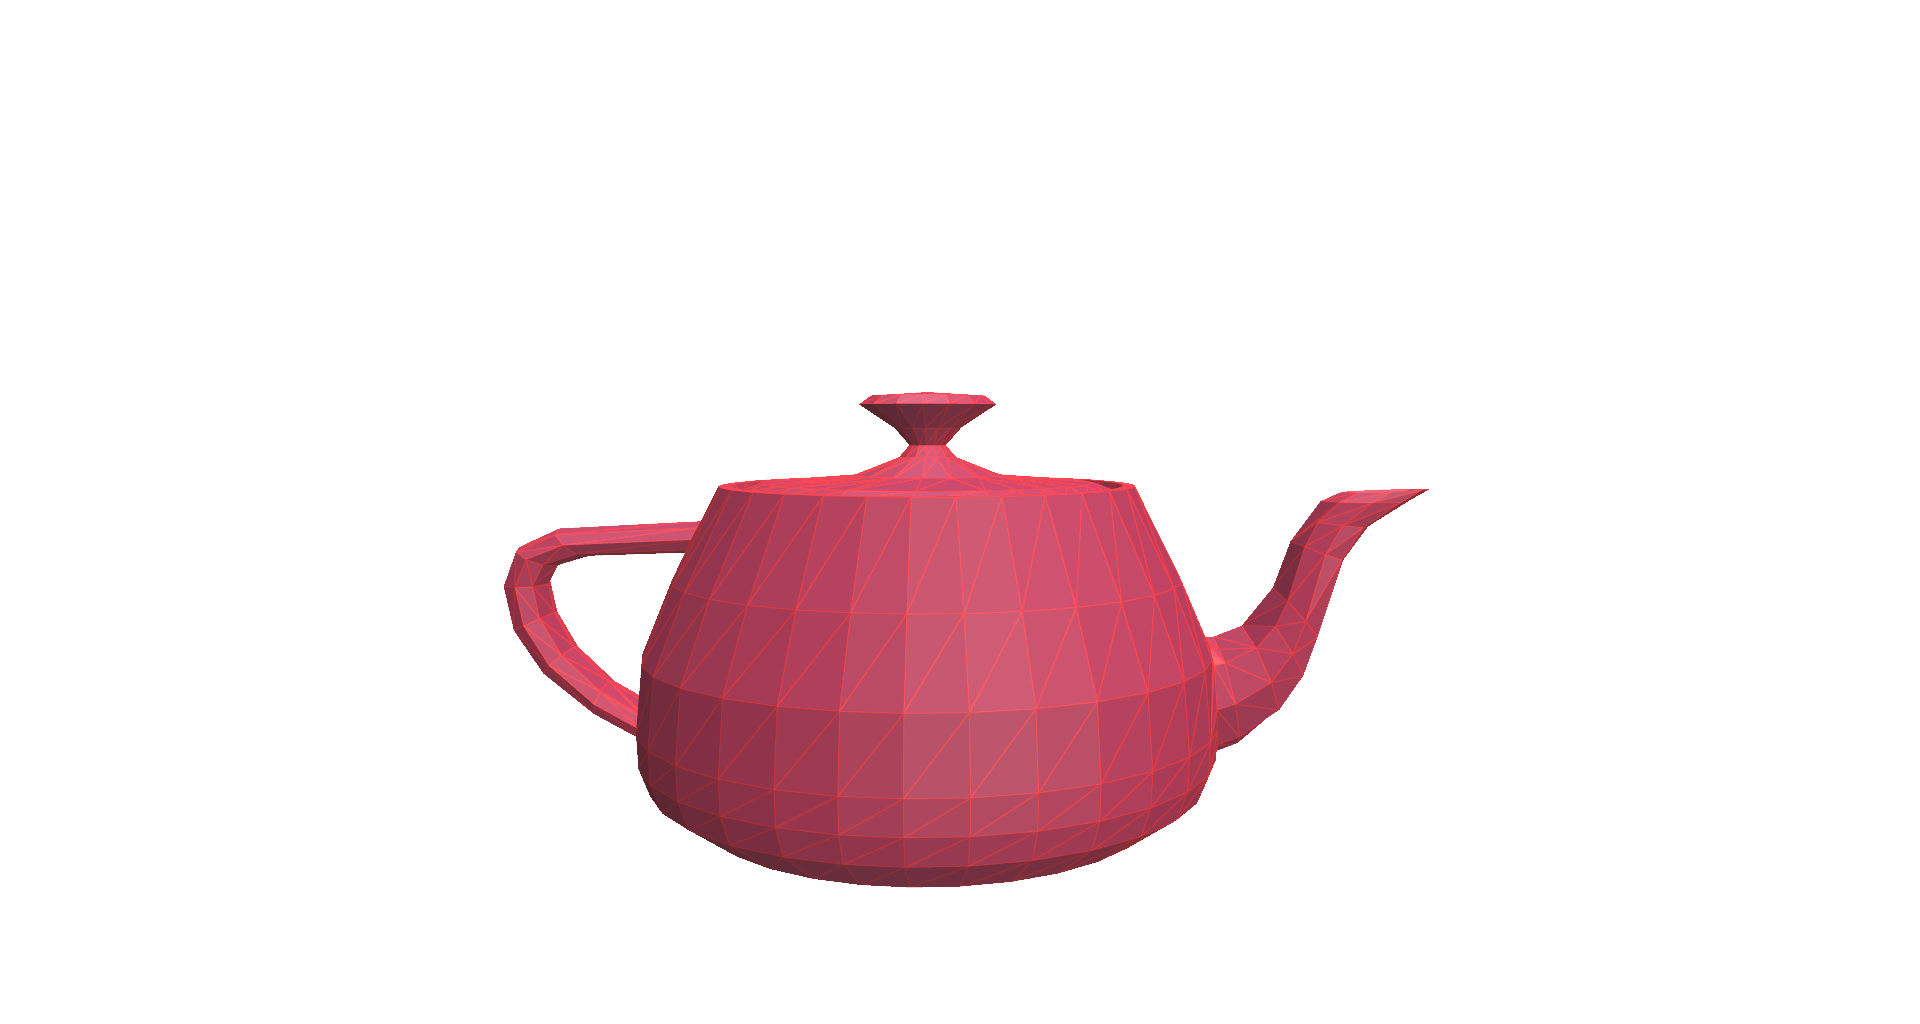
\includegraphics[width=4in]{images/image7.png}
  %\setcapindent{0em}
  \caption{Illustration  der Modellierung von 3D-Objekt durch zweidimensionale Triangulierungen }
\end{figure}

Delaunay-Refinement  mit einer Oberflächentriangulierungen als Eingabe hat die Schwierigkeit, dass im Allgemeinen die durch die Optimierung veränderte  Oberflächentriangulierung die geometrischen Nähe zum Ursprungsobjekt verliert (siehe Abbildung~\ref{fig:extrinsich_kanten_flip}).\\
\begin{figure}[H]%{r}{5cm}
    \centering
    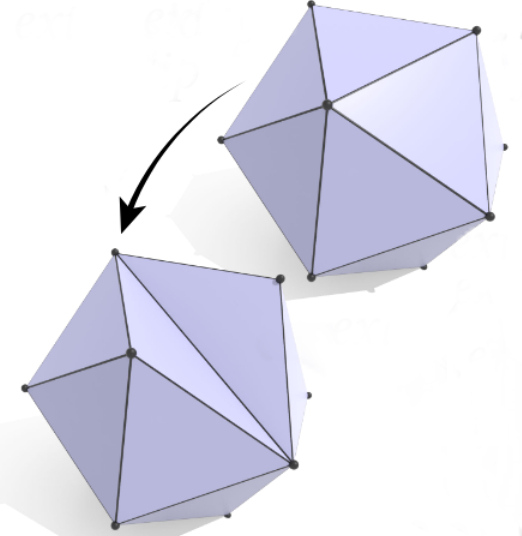
\includegraphics[width=2in]{images/extrinsicher_kantenflip.jpg}
  %\setcapindent{0em}
  \caption{Illustration  dass durch die der Veränderung der Oberflächentriangulierung auch die Geometrie verändert wird~\cite{Sharp:2019:NIT}}
  \label{fig:extrinsich_kanten_flip}
\end{figure}

Beim Intrinsischen Delaunay-Refinement  wiederum wird die Eingabe als Triangulierung einer abstrakten Fläche betrachtet, wodurch nur die Triangulierung selbst verändert wird, nicht aber ihre Lage im Raum. Dadurch bleibt die Geometrie des Objekts trotz Veränderung der Triangulierung erhalten.
In~\cite{Sharp:2019:NIT} stellt~\citeauthor{Sharp:2019:NIT} ein Werkzeug für ein intrinsisches Delaunay-Refinement  vor, das sich ausschließlich auf die Qualität der Triangulierung konzentriert, ohne die zugrunde liegende Geometrie zu verändern (siehe Abbildung~\ref{fig:intrinischer_kanten_flip}).\\  


\begin{figure}[H]%{r}{5cm}
    
    \centering
    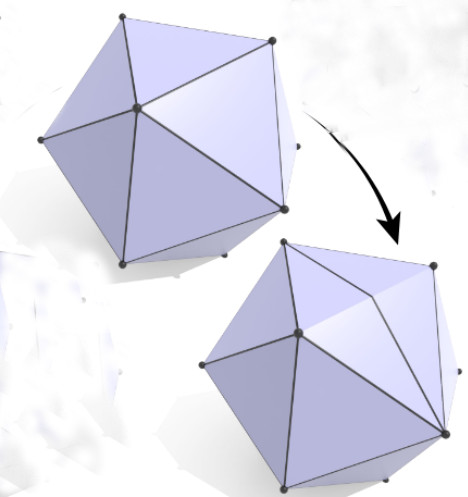
\includegraphics[width=2in]{images/intrinsch_kantenflip.jpg}
  %\setcapindent{0em}
  \caption{Illustration  dass durch intrinsische Veränderung der Oberflächentriangulierung  die Geometrie nicht verändert wird~\cite{Sharp:2019:NIT}}
  \label{fig:intrinischer_kanten_flip}
\end{figure}
\newpage
Das Ziel dieser Bachelorarbeit ist es nun, zu zeigen, welche Einschränkungen bei der Übertragung des Terminierungsbeweises vom planaren Delaunay-Refinement  Verfahren~\cite{chew:1989:guaranteed,ruppert:1995:delaunay,SHEWCHUK:2002:chuws} auf das von  \citeauthor{Sharp:2019:NIT} in   \cite{Sharp:2019:NIT}  vorgestellte intrinsische Delaunay-Refinement  Verfahren auftreten.\\ Dazu werden wir zuerst das traditionelle Delaunay-Refinement  besprechen und vergleichend dazu das intrinsischen Delaunay-Refinement, die Unterschiede zwischen beiden und die daraus resultierenden Schwierigkeiten für den Terminierungsbeweis.\\ 


Der Hauptunterschied liegt hierbei im Winkeldefekt, der bei Oberflächen von Objekten auftreten kann. Ein Winkeldefekt liegt vor, wenn sich die Winkel einer Oberfläche um einen Punkt zu mehr oder weniger als $2\pi$ addieren. Dies kann in der euklidischen Ebene nicht passieren: Hier addieren sich die Winkel um einen Punkt immer genau zu $2\pi$.



Ich zeige in dieser Arbeit, dass ein Winkeldefekt kleiner gleich $\frac{5}{3}$ keine Auswirkungen auf die Terminierung hat. Auf den Umgang mit Segmenten, Größenoptimalität und Aspekte der Abstufung werde ich nur am Rande eingehen.\\











 		\chapter{ Verwandte Arbeiten}


In diesem Kapitel werden einige wissenschaftlichen Arbeiten vorgestellt,
auf denen diese Bachelorarbeit aufbaut.

\citeauthor{SHEWCHUK:2002:chuws}\cite{shewchuk:1997:delaunay,SHEWCHUK:2002:chuws} diskutiert ausführlich die Delaunay-Triangulierung und verschiedene Delaunay-Refinement Algorithmen in der euklidischen Ebene. Eine ausführliche Beschreibung des Delaunay-Refinement ist in Kapitel~\ref{kap:Algorithmus} S.\pageref{kap:Algorithmus} dieser Bachelorarbeit zu finden.
In seinen Arbeiten werden auch die bekanntesten Verfahren von~\citet{chew:1993:guaranteed,chew:1989:guaranteed} und~\citet{ruppert:1995:delaunay} vorgestellt.
Da die Triangulierungen von geschlossenen stückchenweise flachen Oberfläche (StF-Oberflächen) keine Segmente enthält, wird in dieser Bachelorarbeit nicht weiter auf den Unterschied der beiden Algorithmen eingegangen. Siehe dazu und zum jeweiligen Umgang mit Segmenten: \citeauthor{shewchuk:1997:delaunay}.\\
\begin{figure}[ht]%{r}{5cm}
    \centering
  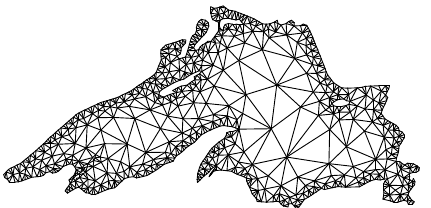
\includegraphics[width=3in]{images/tripslg.png}
  %\setcapindent{0em}
  \caption{Illustration des Delaunay-Refinement:
  Für das abgebildete Polygonzug erzeugt Chew zweite und Ruperts Version fast die gleiche Ausgangstriangulierung~\cite{SHEWCHUK:2002:chuws}.}
\end{figure} 

Analog zur Triangulierung von Flächen in der euklidischen Ebene beschäftigen wir uns mit der Triangulierung~\cite{Bobenko:2007:LaplaceBeltrami} von Flächen, die im dreidimensionalen Raum eingebettet sind. Diese werden in der Mathematik  vereinfachte als stückchenweise flache 2-Mannigfaltigkeiten  \cite{betke:1984:2-Mannigfaltigkeiten} bezeichnet.
\citeauthor{SHEWCHUK:2002:chuws} vermutet dazu, dass sich die Lemmata, welche für Triangulierungen gelten, übertragen lassen~\cite[Abschnitte 5.3.2]{SHEWCHUK:2002:chuws}. Diese Übertragbarkeit werden wir in Kapitel~\ref{kap:Terminierung}  auch für einige Lemmata von~\citet{ruppert:1995:delaunay} zeigen.\\  

Diese Arbeit orientiert sich an der Definition von~\citet{Bobenko:2007:LaplaceBeltrami}, die auf den Arbeiten~\cite{boris1934delaunay,indermitte:2001:voronoi,lambert:1994:delaunay} aufbaut. Sie zeigen in ihrer Arbeit, dass die Eigenschaften, die für die Delaunay-Triangulierung in der Ebene gelten, sich auch auf die Delaunay-Triangulierung  von stückchenweise flachen Oberflächen~\cite[Definiton 1] {Bobenko:2007:LaplaceBeltrami}  im dreidimensionalen Raum übertragen lassen~\cite[Definition 3]{Bobenko:2007:LaplaceBeltrami}.\\

Von~\citet{Bobenko:2007:LaplaceBeltrami} inspiriert entwickeln~\citet{Bobenko:2006:SIGGRAPH} das \textit{incremental overlay-Schema} \cite[Abschnitt 2.3]{Bobenko:2006:SIGGRAPH}. Das Schema basiert auf dem expliziten Speichern von Kantenschnittpunkten und ist die erste Datenstruktur zur Realisierung intrinsischer Triangulierungen. Das \textit{incremental overlay-Schema} wurde gezielt für intrinsische Kantenflips entwickelt und unterstützt darüber hinaus nur wenige weitere Operationen~\cite[Abschnitt 2]{Sharp:2019:NIT}. \\
\begin{figure}[ht]%{r}{5cm}
    \centering
  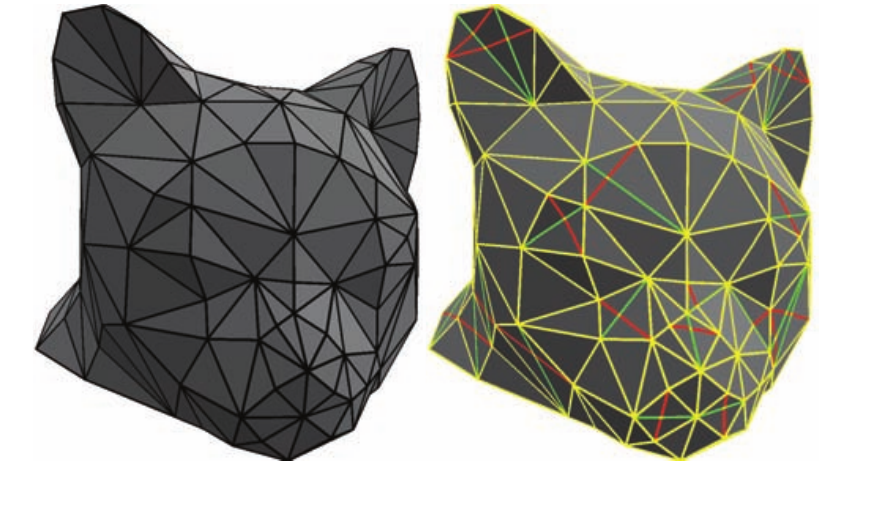
\includegraphics[width=3in]{images/overlaySchema.png}
  %\setcapindent{0em}
  \caption{Illustration des \textit{incremental overlay-Schema}:  Original kanten \textcolor{green}{grüne} geflipte Kanten \textcolor{red}{rot} und nicht veränderte kanten \colorbox{gray}{\textcolor{yellow}{gelb}}. Gespeichert werden die Schnittpunkte der Kanten.  \cite{Bobenko:2006:SIGGRAPH}}
\end{figure}
    
\citet{Sharp:2019:NIT} hat mit der \textit{signpost data structure} eine allgemeinere Datenstruktur vorgestellt~\cite[Abschnitt 3]{Sharp:2019:NIT}, welche weitere Operationen auf intrinsischen Triangulierungen ermöglicht. Mithilfe dieser Datenstruktur gelingt es ihm unter anderem, eine intrinsische Version des Delaunay-Refinement Verfahrens für Triangulierungen in der euklidischen Ebene auf Triangulierungen von stückchenweise flachen Oberflächen~\cite[Definition 1]{Bobenko:2007:LaplaceBeltrami} anzuwenden. 
 \begin{figure}[ht]%{r}{5cm}
    \centering
  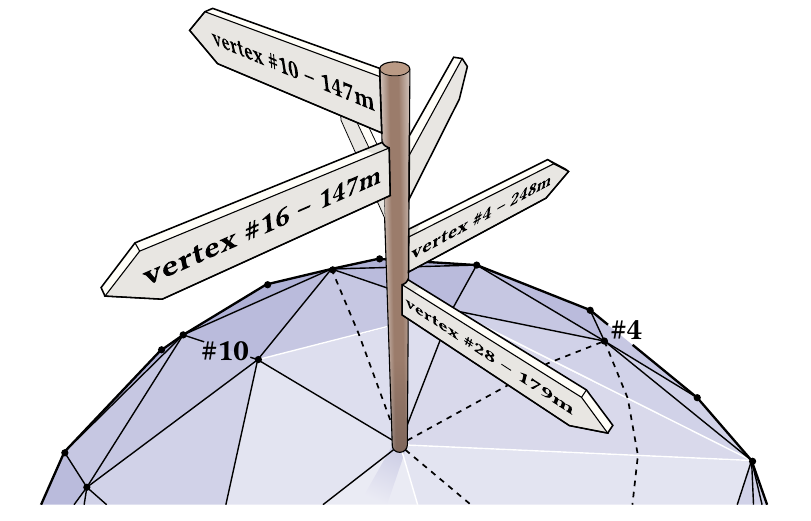
\includegraphics[width=3in]{images/signpostDataStructure.png}
  %\setcapindent{0em}
  \caption{Illustration des \textit{signpost data structure}: Sie basiert auf einer Halbkanten-Datenstruktur~\cite{mantyla:1987:halfedge}, die  Triangulierungen implizit codiert, indem sie die Richtung und den Abstand benachbarter Knoten speichert. Diese implizite Codierung ermöglicht die praktische Anwendung des intrinsischen Delaunay-Refinement.  \cite{Bobenko:2006:SIGGRAPH}}
\end{figure}
Das intrinsische Delaunay-Refinement von~\citeauthor{Sharp:2019:NIT} basiert auf dem zweiten Algorithmus von~\citet{chew:1993:guaranteed}, mit der Modifikation, dass Dreiecke, die einen Knoten von Grad Eins enthalten, ignoriert werden. 
Da~\cite{Sharp:2019:NIT} zur Unterstützung seiner These nur eine empirische Betrachtung vornimmt, ist noch nicht gesichert, dass der Algorithmus mathematisch korrekt ist und für jede Eingabe terminiert. Diese Bachelorarbeit beschäftigt sich daher mit dem Beweis, dass das intrinsische Delaunay-Refinement terminiert.\\

Es folgen nun weitere Möglichkeiten für Refinement-Verfahren, welche jedoch nicht Teil dieser Bachelorarbeit sind.

\citet{ungoe:2004:off-center} stellt das Delaunay-Refinement mit \textit{off-center}-Einfügestrategie vor, die eine Verallgemeinerung der Umkreismittelpunkt-Einfügestrategie ist.

\citet{rand:2011:Miller-Pav-Walkington} zeigte bereits mithilfe der \textit{Miller-Pav-Walkington analysis}, dass im zweidimensionalen Raum bessere Ergebnisse erzielt werden als mit dem bekannten Delaunay-Refinement.
Weitere Möglichkeiten hierfür sind auch die optimale Delaunay-Triangulierung von Chen und Xu~\cite{chen:2004:mesh-odt,chen:2004:optimal-delaunay-triangulation} und die Minimal-Gewichtete-Triangulierungen von~\citet{mulzer:2008:minimum}.

Die genannten Algorithmen ließen sich mit der von~\citet{Sharp:2019:NIT} vorgestellten Datenstruktur auch leicht in eine intrinsische Form bringen.\\

Der Vollständigkeit halber werden an dieser Stelle noch andere Arbeiten genannt, die sich mit alternativen intrinsischen \textit{remeshing} beschäftigt haben. \citet{liu:2017:geodesic_Voronoi} und~\citet{xin:2011:geodesic_delaunay} haben die intrinsische Delaunay-Triangulierung mithilfe  geodätischer Methoden erzeugt. Der Vorteil dieser Methode ist, dass die Ausgabe eine extrinsisches Triangulierung ist. Der Nachteil ist laut~\citet{Sharp:2019:NIT}, dass unter Umständen viele Elemente erzeugt werden können und die Triangulierung zwar Delaunay-Eigenschaften hat, jedoch immer noch kleine Winkel aufweisen kann.\\ %Alt: 
  		\chapter{ Grundlagen}
Diese Arbeit befasst sich mit Winkeldefekten und ihren Auswirkungen auf die Terminierung des intrinsischen Delaunay-Refinement. Zum Verständnis sind Grundkenntnisse der computergestützten Geometrie und deren Begrifflichkeiten sowie allgemeine mathematische Grundbegriffe erforderlich. Im Folgenden werden daher einige der wichtigsten Grundbegriffe und Definitionen erläutert. Wir orientieren uns dabei in der
Formulierung an den Arbeiten von 
 Bobenko, Springborn, Fisher u. a., Sharp u. a. und Shewchuk
 \cite{Bobenko:2006:SIGGRAPH,Sharp:2019:NIT,Bobenko:2007:LaplaceBeltrami,shewchuk:1997:delaunay,SHEWCHUK:2002:chuws},
wobei wir die Notation im Sinne der Konsistenz dieser Arbeit ggf. anpassen.

\section*{Triangulierung}

Eine Triangulierung $M$, gegeben durch das Tripel $  (V, E, T) $, ist die Zerlegung einer Fläche oder Oberfläche in disjunkte Dreiecksflächen; die Dreiecke sind dabei entlang ihrer Kanten überlappungsfrei verbunden.
Triangulierungen bestehen dabei im Allgemeinem nicht aus uniformen Dreiecken.
Die Vereinigung der disjunkten Dreiecksflächen bildet die zerlegte Fläche. \\  

\begin{figure}[h]%{r}{5cm}
    \centering
  \input{figuren/zulässige_triangulierungen}
  %\setcapindent{0em}
  \caption{Illustration von zulässigen und nicht zulässigen Flächenaufteilungen}
\end{figure}

Dabei bezeichnet  $V$ die Menge der Knoten, $E$ die Menge der Kanten und $T$ die Menge der Dreiecksflächen.


\section*{Auffaltung}
Die Auffaltung eines dreidimensionalen Objektes ist die Ausbreitung der Flächen seiner Oberfläche (oder Teilen davon) in der euklidischen Ebene, nachdem es an einigen Kanten aufgeschnitten worden ist. 

\section*{Gesamtwinkel}
\label{def:gesamtwinkel}
Seien $M = (V, E, T)$ eine Triangulierung, $i,j,k \in V$ und $(i, j),(i, k),(j, k) \in E$, dann bezeichnet $\theta_i^{j,k}$ den Winkel zwischen den Kanten  $(i, j)$ und $(i, k)$ in einem Dreieck. Der Gesamtwinkel $ \Theta_i$ eines Knotens $i$ bezeichnet die Summe aller zu $i$ gehörender Innenwinkel $\theta_i^{j,k}$.

\begin{figure}[H]%{r}{5cm}
    \centering
  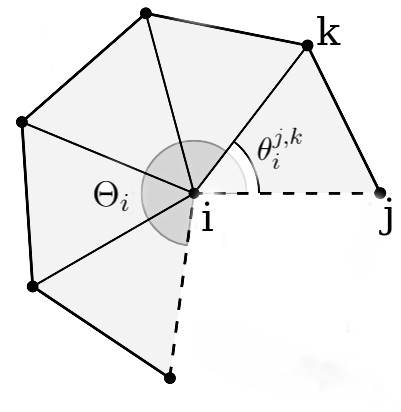
\includegraphics[width=2in]{images/gesammtwinkel.jpg}
  %\setcapindent{0em}
  \caption{Illustration Gesamtwinkel \gesamtwinkel und Innenwinkel  $\theta_i^{j,k}$  eines Knotens $i$  \cite{Sharp:2019:NIT}}
\end{figure}
 
\section*{Winkeldefekt}
\label{def:winkeldefekt}
In der euklidischen Ebene addieren sich die Winkel um einen Knoten zu $2\pi$. Bei einer Oberfläche können die Winkel sich zu weniger oder mehr als $2\pi$ addieren.\\
Dieses Phänomen bezeichnet man in der Geometrie als Winkeldefekt. Für den Gesamtwinkel eines Knotens gilt dann: $\gesamtwinkel* \neq 2\pi$ 

\cite{richeson:2012:euler}.\\
\begin{figure}[H]%{r}{5cm}
    \centering
  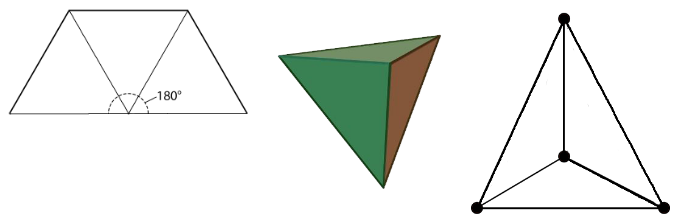
\includegraphics[width=4in]{images/winkeldefekt_polyder_2.png}
  %\setcapindent{0em}
  \caption{Illustration eines Knotens mit Gesamtwinkel $\pi$ und  Winkeldefekt von $\pi$ \cite{Koch_2019_CVPR}}
\end{figure}
 
 Bei einer Oberfläche ist der Winkeldefekt an einem Knoten $i$ gleich $2\pi - \gesamtwinkel* $. 

\begin{definition}(Kegelspitze)\\

Ein Knoten $s \in V$  wird als Kegelspitze bezeichnet, wenn er einen Winkeldefekt hat.\\
 
Es werden zwei Arten von Kegelspitzen unterschieden:
 \begin{itemize}
     \item sphärische Kegelspitzen, falls $\Theta_s < 2\pi $ und 
     \item hyperbolische Kegelspitzen, falls $\Theta_s > 2\pi $.
 \end{itemize} 


\begin{figure}[h]%{r}{5cm}
    \centering
  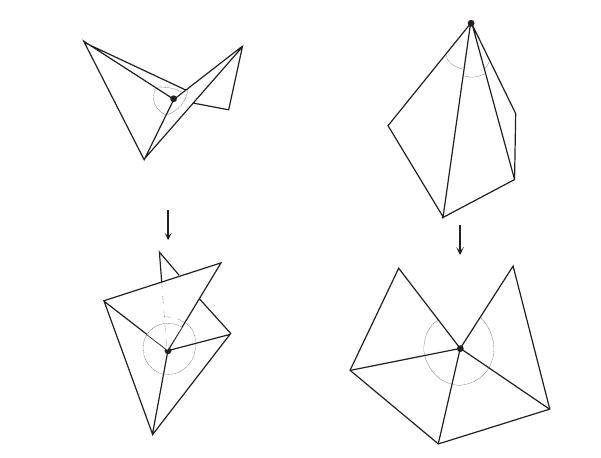
\includegraphics[width=3in]{images/Merged_document.png}
  %\setcapindent{0em}
  \caption{Links hyperbolische Kegelspitze und rechts sphärische Kegelspitze   \cite{Polthier:2006:SIGGRAPH}}
\end{figure}
 

\end{definition}

\section*{Delaunay-Triangulierung einer stückchenweise flachen Oberfläche}
\begin{figure}[H]%{r}{5cm}
    \centering
    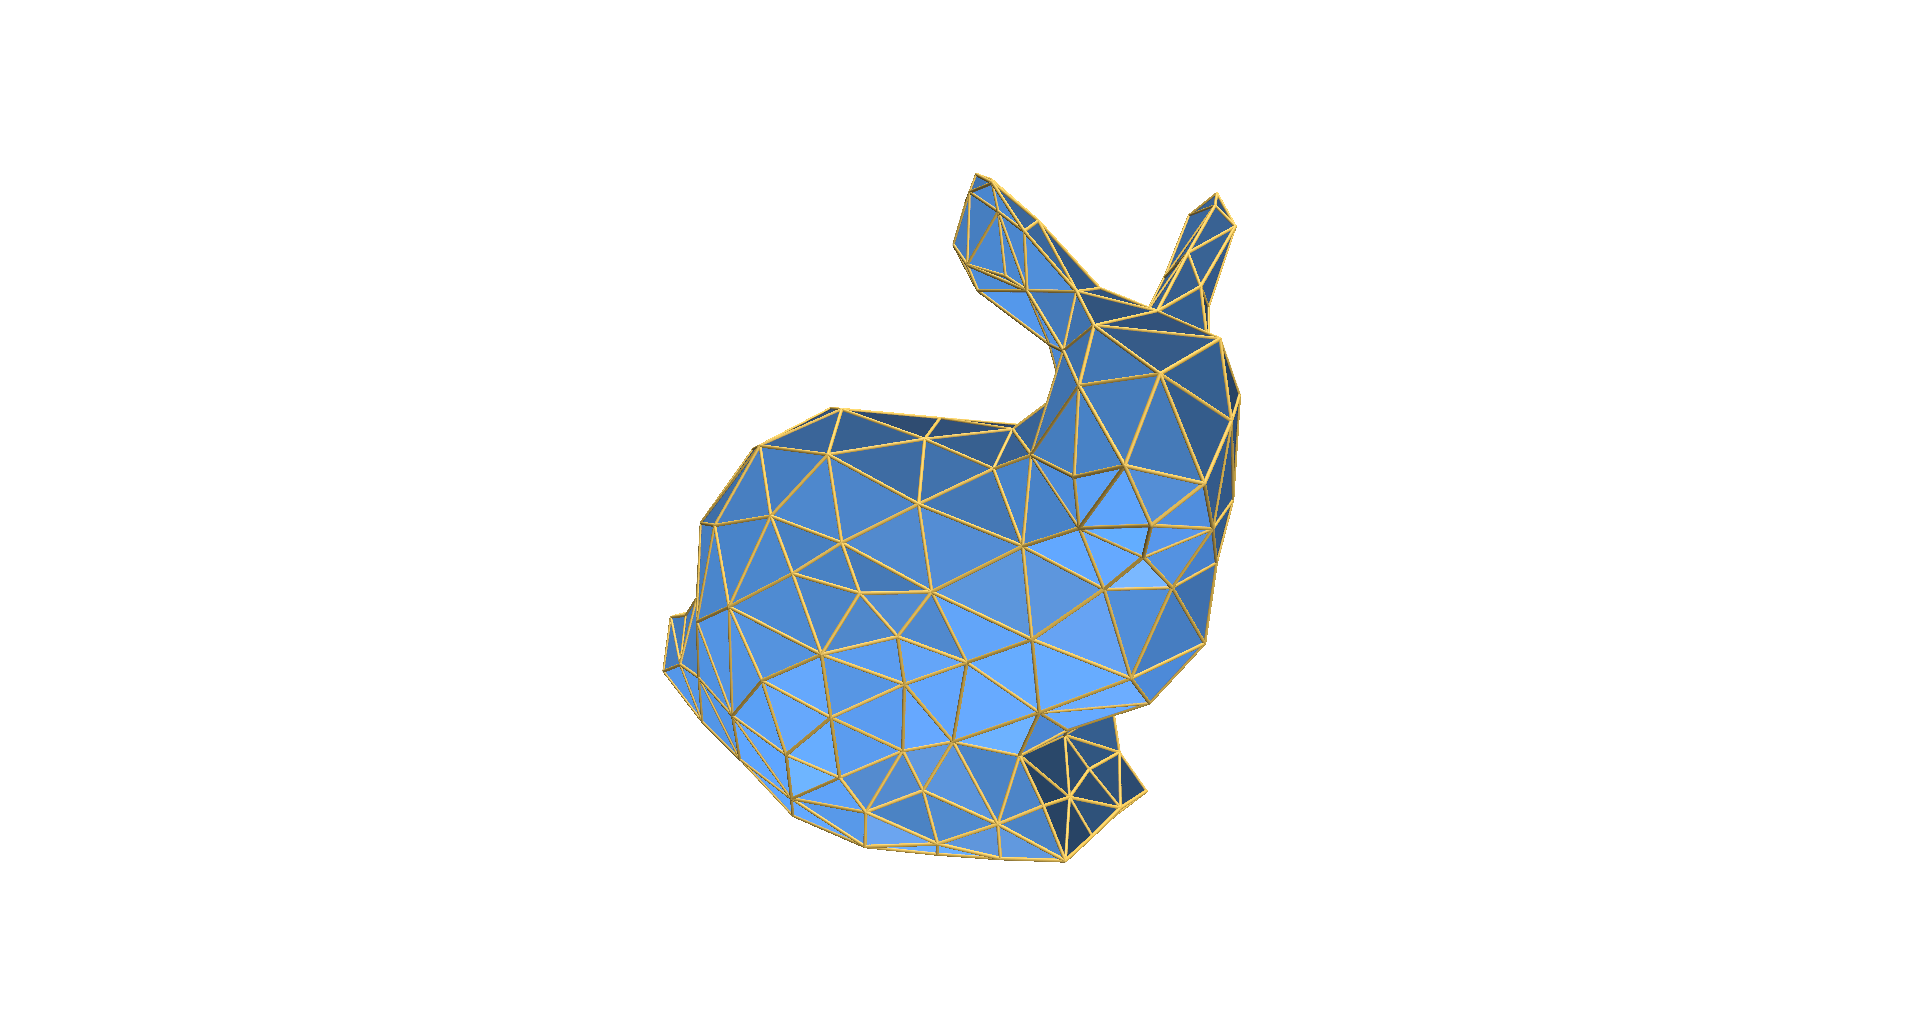
\includegraphics[width=5in]{images/image1.png}
  %\setcapindent{0em}
  \caption{Illustration der Triangulierung einer stückchenweise flachen Oberfläche}
   \label{fig:hase}
\end{figure}

\subsection*{Stückchenweise flache Oberflächen (StF-Oberflächen)}

Stückweise flache Oberflächen wie in Abbildung~\ref{fig:hase} gezeigt sind 2-Mannigfaltigkeit mit kegelspitzenartigen Singularitäten. Intuitiv bedeutet das, dass diese Flächen lokal euklidisch sind außer an einigen singulären Punkten. Dort verhalten sie sich wie eine sphärische oder hyperbolische Kegelspitze. Kegelspitzen können im Allgemeinen dort auftreten, wo Linien zusammengeführt werden (siehe Abbildung~\ref{fig:hase}).

\subsection*{Triangulierung  einer  StF-Oberfläche}
Sei $M = (V,E,T)$ eine Triangulierung einer StF-Oberfläche. Dann gilt für die Menge der Kegelspitzen $S$ der StF-Oberfläche, dass $S \subset V$.\\ 
 
Die Triangulierung einer Stf-Oberfläche ist für gewöhnlich eine Sammlung von ebenen Dreiecken im Raum (siehe Abbildung~\ref{fig:hase}). Dies ist jedoch keine Anforderung an die Triangulierung, es wird lediglich gefordert, dass die Möglichkeit existiert, jede Fläche als Dreieck in der euklidischen Ebene aufzufalten. \\  

Auf $M$ sind also auch sogenannte irreguläre Dreiecke erlaubt, bei denen (zum Beispiel) ein Knoten eine (irreguläre) Kante zu sich selbst hat und die anderen beiden Kanten gleich sind oder alle drei Knoten identisch sind (siehe Abb. \ref{fig:auffaltung_irregulaer}).
Formal ist $M$  somit ein $\Delta$-Komplex~\cite[Abschnitt 2.1]{hatcher:2005:deltakomplex}.\\
 
\begin{figure}[H]%{r}{5cm}
    \centering
  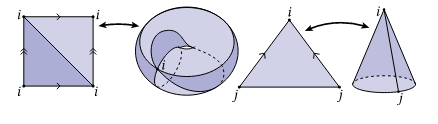
\includegraphics[width=4in]{images/auffaltung_irregulaer.png}
  %\setcapindent{0em}
  \caption{Illustration von irregulären Dreiecken, die sich in der  euklidischen Ebene zu gewöhnliche Dreiecken auffalten~\cite{Sharp:2019:NIT}}
\label{fig:auffaltung_irregulaer}
\end{figure}
% in der Geometrie bezieht sich intrinsische darauf, dass (zum Beispiel) Oberflächen ohne Bezug auf ihre Lage im Raum beschrieben werden, wobei nur Messungen entlang der Oberfläche (Längen, Winkel usw.) verwendet werden.\\


\begin{definition}(Eingebettete leere Kreisscheibe)\\
Sei $M = (V,E,T)$ eine Triangulierung einer StF-Oberfläche.
Eine eingebettete leere Kreisscheibe ist eine stetige Abbildung $\phi: k^{\ast} \rightarrow M$, wobei $k$ eine offene runde Scheibe in der euklidischen Ebene und  $k^{\ast}$ ihr Abschluss ist.
Jeder $v \in K$ hat eine Nachbarschaft, die isometrisch abgebildet wird. Es gilt $\phi (k) \cap V = \emptyset $. Folglich sind alle Punkte in $\phi^-1(V)$ im Rand von $K$ enthalten: $\phi^{-1}(V) \subset \partial K $ 
\end{definition} 
 
 
 

\subsection*{Delaunay-Triangulierung einer geschlossenen StF-Oberfläche}
Sei $M = (V,E,T)$ eine Delaunay-Triangulierung einer geschlossenen StF-Oberfläche.
Die Delaunay-Triangulierung ist dabei eine Zerlegung der StF-Oberfläche in disjunkte Teilmengen und besteht aus folgenden Mengen: Eine Teilmenge $ C \subset M$ ist eine geschlossene Zelle der Delaunay-Triangulierung genau dann, wenn eine eingebettete leere Kreisscheibe $\phi: k^{\ast} \rightarrow M$ existiert, sodass $\phi^{-1}(M) \not = \emptyset$ und auf ihrem Rand genau die Elemente aus $C$ liegen. 
$C$ ist also das Bild der konvexen Hülle von $\phi^{-1}(M)$.
Dabei unterscheidet man die Zellen an der Anzahl ihrer Knoten: 1-Zellen (Knoten), 2-Zellen (Kanten) und 3-Zellen (Flächen).\\   

Aufgrund ihrer nützlichen Eigenschaften ist die  Delaunay-Triangulierung  eine der in der Praxis am häufigsten eingesetzten Triangulierungen. 
Die Eigenschaften sind unter anderem:

\begin{itemize}
    \item die Dualität zum Voronoidiagramm (siehe Abb. \ref{fig:delaunay_voronoi}  ) \cite{indermitte:2001:voronoi,aurenhammer:2000:voronoi}
    \item die Eigenschaft der leeren Kreisscheibe (im folgenden Delaunay-Eigenschaft genannt)\\(siehe Abb. \ref{fig:delaunay_umkreis})
    \item sie ist in der Regel eindeutig (siehe Abb. \ref{fig:eindeutig})
    \item jede beliebige Triangulierung kann mit einer endlichen Zahl an Kantenflips in eine Delaunay-Triangulierung überführt werden. Dies gilt für die euklidische Ebene~\cite{shewchuk:1997:delaunay} und für die StF-Oberfläche~\cite{Bobenko:2007:LaplaceBeltrami}.
    \item eine Kante ist genau dann Teil der Delaunay-Triangulierung,  wenn sie die Delaunay-Eigenschaft erfüllt. 
    \item unter allen möglichen Triangulierungen ist die Delaunay-Triangulierung diejenige, welche den minimalen Innenwinkel über alle Dreiecke maximiert. 
    %\item die Maximierung des minimalen Innenwinkels über alle Dreiecke. Letztere Eigenschaft verhindert in weiterer Folge Rundungsfehler.
\end{itemize}
 
 
 \begin{figure}[H]
    \centering
    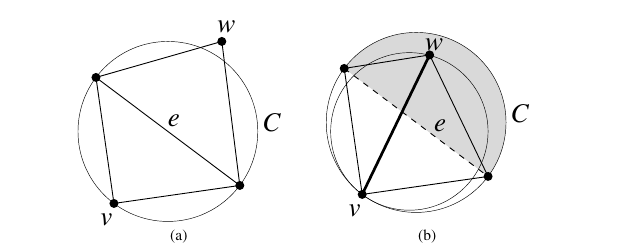
\includegraphics[width=5in]{images/lokal_delaunay.png}
    \caption{Illustration: dass jede Kante, Kante die geflippt werden muss geflipt werden kann. in $(a)$ erfüllt $e$ die Delaunay-Eigenschaft. in $(b)$ erfüllt $e$ sie nicht kann, aber die durch den Kantenflip erzeugt Kante erfüllt die Delaunay-eigenschaft~\cite{shewchuk:1997:delaunay} }
    \label{fig:lokal_delaunay}
\end{figure}


\begin{figure}[h]%{r}{5cm}
    \centering
  \includesvg[width=2in]{images/Delaunay_Voronoi}
  %\setcapindent{0em}
  \caption{ Umkreismittelpunkte der Dreiecke der Delaunay-Triangulierung sind die Knoten  der Voronoizellen.\cite{Hferee:2011:delaunay-voronoi}}
  \label{fig:delaunay_voronoi}
\end{figure}

\begin{figure}[H]%{r}{5cm}
    \centering
  \includesvg[width=2.5in]{images/Delaunay_circumcircles}
  %\setcapindent{0em}
  \caption{Der Umkreis eines Dreiecks ist die einzige Kreisscheibe, die durch die drei Eckknoten des Dreiecks verläuft. Die Delaunay-Triangulierung ist die Triangulierung, bei der jedes Dreieck einen leeren Umkreis (Kreisscheibe) besitzt. D. h. die Fläche der Kreisscheibe enthält keine anderen Knoten der Triangulierung. \cite{Gjacquenot:2013:delaunay-circumcircles}}
  \label{fig:delaunay_umkreis}
\end{figure}
    
    
\begin{figure}[H]
    \centering
    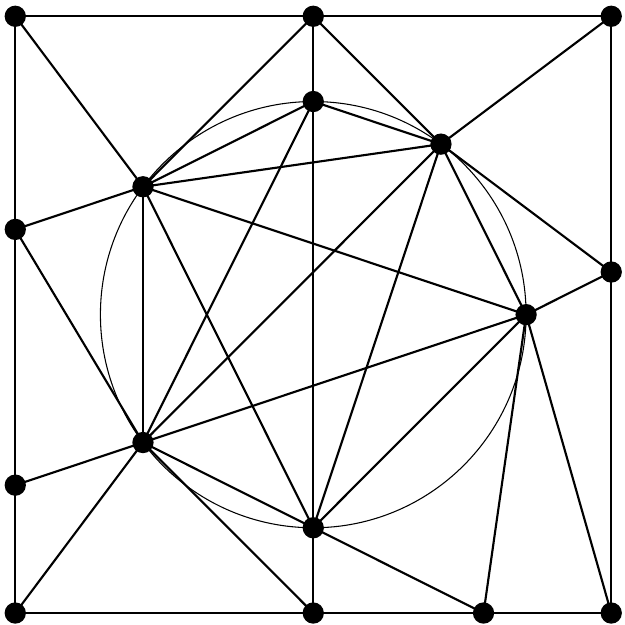
\includegraphics[width=2in]{images/Bildschirmfoto von 2021-11-27 22-34-40.png}
    \caption{ Wenn mehr als drei Punkte auf dem Rand derselben Kreisscheibe liegen, ist die Delaunay Triangulierung nicht eindeutig. Da dies in der  Praxis selten vorkommt, treffen wir die vereinfachte Annahm, dass niemals mehr als drei Punkte auf einer Kreisscheibe liegen~\cite{shewchuk:1997:delaunay} }
    \label{fig:eindeutig}
\end{figure}
    
\newpage

Die Qualität der Triangulierung definiert sich über das Verhältnis der  Innenwinkel- und Flächenverteilung der einzelnen Dreiecke. 
Da die durch die Delaunay-Triangulierung maximierten Innenwinkel über alle Dreiecke einer festen Knotenmenge noch zu klein sein könnten, 
kann die Qualität darüber hinaus verbessert werden. Dies kann über das gezielte Einfügen weiterer Knoten geschehen. Hierfür werden Delaunay-Refinement Algorithmen verwendet.\\

 






  		\chapter{ Delaunay-Refinement }\label{kap:Algorithmus} Da der Schwerpunkt dieser Arbeit auf dem Terminierungsbeweis des intrinsischen Delaunay-Refinement liegt, wird im Folgenden das Delaunay-Refinement vorgestellt und eine intuitive Beweisidee geliefert. Die Ausführungen beruhen dabei auf den Überlegungen von \citet{shewchuk:1997:delaunay,SHEWCHUK:2002:chuws}.\\
Delaunay-Refinement Algorithmen basieren auf Delaunay-Triangulierung, die so lange durch das Einfügen neuer Knoten optimiert werden, bis die Triangulierung die vorher definierten Anforderungen an Winkel- und Flächengröße erfüllt. In diesem Kapitel wird davon ausgegangen, dass der Leser mit Delaunay-Triangulierungen vertraut ist; für weiter Informationen siehe Lee, Lin \cite{lee:1986:DelaunayTriangulation} und \citet{chew:1993:guaranteed}. 


\section*{Beschreibung des Algorithmus}
%Zu den bekanntesten Delaunay-Refinement-Methoden gehören die Algorithmen von \citet{chew:1993:guaranteed,chew1989guaranteed} und der von Ruppert \cite{ruppert:1995:delaunay}. Da die Triangulierung einer geschlossenen StF-Oberfläche in der Regel keine Segmente enthält, sparen wir uns die Behandlung von Segmenten. Mehr Information zum Umgang siehe \cite{SHEWCHUK:2002:chuws}.\\

Delaunay-Refinement-Algorithmen bestehen üblicherweise aus zwei Schritten: das Einfügen eines neuen Knotens und die Wiederherstellung der Delaunay-Eigenschaft.
Diese Schritte  werden so lange wiederholt, bis die Triangulierung die vorher definierten Anforderungen erfüllt.\\ 
   %Delaunay-Refinement-Algorithmen, die als Eingabe keine Delaunay Triangulierung bekommen, haben für gewöhnlich noch den zusätzlichen Schritt die Eingabe zu Triangulieren und ggf. die Delaunay Eigenschaft herzustellen.  
%   Der Algorithmus von \citet{chew:1993:guaranteed} wird hier mit einigen Änderungen gegenüber dem ursprünglichen Algorithmus vorgestellt. Die wichtige Änderung ist, dass der Algorithmus als Eingabe: Triangulierungen von geschlossenen StF-Oberfläche hat.
  
%   Die Triangulierung einer geschlossenen StF-Oberfläche enthält in der Regel keine Segmente.
%   dadurch, benötigen wir auch keine eingeschränkte Delaunay Triangulierung und sparen uns die Behandlung von Segmenten.
  % Die  Delaunay-Triangulierung kann nur eine feste Knotenmenge optimal zu einem Dreiecksnetz verbinden. Möchte man darüber hin die Qualität der Triangulierung, die Innenwinkel oder Flächenaufteilung der einzelnen Dreiecke verbessern, kann dies über das gezielt einfügen weiter Knoten  geschehen.
% Aufgrund ihrer nützlichen Eigenschaften ist die  Delaunay-Triangulierungen $M^D$ eine, der in der Praxis am häufigsten eingesetzten Triangulierungen. die Eigenschaften sind z.b. die Dualität zum Voronoi Diagramm, dass eine Kante, genau dann Teil der Triangulierung ist  wenn sie eine leere Kreisscheibe Besitz, Sodas nur die Endknoten der Kante auf den Rand der Scheibe liegen und die Maximierung des minimalen Innenwinkels über alle Dreiecke. Letztere Eigenschaft verhindert in weiterer Folge
% \begin{definition}(Umkreisradius-zu-kürzester-Kante Verhältnisses).\\
% \label{def:UrzkK}
% Das Umkreisradius-zu-kürzester-Kante-Verhältnis im Folgenden \UrzkK ist eine Metrik zur Bewertung von Dreiecksqualität. Die Metrik beschreibt, die Beziehung $\frac{\kuezesteKante*}{2 \umkreisradius*}$  zwischen dem Umkreisradius \umkreisradius eines Dreiecks und der Länge seiner kürzesten Kante \kuezesteKante.\\
% Das Verältniss kann dabei von Delaunay-Refinement Algorithmen  nur verkleinert werden \cite{MiTaTeWa1995ACM}. In [TODO-Kapitel-Referenz] zeigen wir, dass es für Intrinsischen Delaunay Refinement eine natürliche Untergrenze für \UrzkK gibt.\\
% \end{definition}


 \begin{figure}[h]
    \centering
    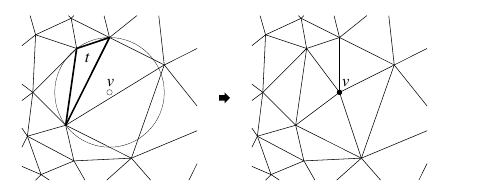
\includegraphics[width=5in]{images/delaunay_refinement.png}
    \caption{Illustration einer Iteration des Delaunay-Refinement: ein dünnes Dreieck $t$ wird geteilt, indem sein Umkreismittelpunkt $v$ eingefügt wird und die Delaunay Eigenschaft der Triangulierung wiederhergestellt wird. \cite{SHEWCHUK:2002:chuws} }
    \label{fig:Punkt_einfügen}
\end{figure}



Die Anforderung an die Eingabe ist für gewöhnlich,
dass alle Innenwinkel der Dreiecke größer als ein Winkel-Schwellenwert \kleinsterWinkel sind.
In Kapitel \ref{kap:Terminierung} zeigen wir, dass der Algorithmus für ein $\kleinsterWinkel* \leq \frac{\pi}{6} $  terminiert.\\
Im Kontext von Delaunay-Refinement werden in der Literatur  Dreiecke als dünn bezeichnet, die die vorher definierten Anforderungen nicht erfüllen \cite{shewchuk:1997:delaunay}. 
Dünne Dreiecke sind z. B. Dreiecke mit mindestens einem Innenwinkel kleiner als \kleinsterWinkel. 

\subsection*{Intrinsischer Delaunay-Refinement Algorithmus}
\textbf{Eingabe:}
Ein Winkel-Schwellenwert \kleinsterWinkel und eine Triangulierung einer StF-Oberfläche, die verfeinert werden soll.  \\

\textbf{Ausgabe:}
Eine intrinsische Delaunay-Refinement derselben StF-Oberfläche, die mit der Geometrie der Eingabe übereinstimmt und keine dünnen Dreiecke mehr enthält.\\

\begin{algorithm}[H]
\label{alg:1}
\SetAlgoLined
\KwData{Triangulierung einer StF-Oberfläche $M$; Winkel-Schwellenwert \kleinsterWinkel }
\KwResult{Intrinsische Delaunay-Refinement  $M^\prime $ }
  WiederherstellenDerDelaunayEigenschaft($M$)\;
 $T_{bad} \gets  \{t_{bad} \in M | t_{bad}  \text{ ist ein dünnes Dreieck}\}$ \;
 \While{$T_{bad} \neq \emptyset$}{
    $t_{bad} \gets T_{bad}$.pop \;
    %$u \gets $Umkreismittelpunkt($t_{bad}$)\;
    EinfügenNeuerKnotens($t_{bad}$, $M$)\;
    %EinfügenEinesNeuenKnotens($t_{bad}$.umkreismittelpunkt, $M$)\;
  WiederherstellungDelaunay-Eigenschaft($M$)\;
  Aktuallisiere($ T_{bad}  $)\;
 }
 \caption{\algorithmusname}
\end{algorithm}


\subsection*{Einfügen neuer Knoten}
Im Allgemeinen liegt der neu einzufügende Knoten $p$ innerhalb der Fläche eines beliebigen Dreiecks  $t$  von $M$, mit $i,j,k \in t$. Dann wird nach dem Einfügen von $p$ in $M$ $t$ aus $M$ entfernt und die Dreiecke $t_{i,j,p}, t_{i,k,p}$ und $t_{k,j,p}$ werden  in $M$ eingefügt. 
Für den Fall, dass $p$ auf einer Kante $e$ liegen, wird derselbe Prozesse auf den beiden angrenzenden Dreiecke ausgeführt (siehe \ref{fig:Punkt_einfügen}).  

 \begin{figure}[h]
    \centering
    \includegraphics[width=3in]{images/Punkt_einfügen_2}
    \caption{Illustration des Punkteinfügens\cite{Sharp:2019:NIT} }%\cite{shewchuk:1997:delaunay}}
    \label{fig:Punkt_einfügen}
\end{figure}
 
 
Der Einfachheit halber wird das Einfügen eines Knotens in den Umkreisradius eines Dreiecks im Folgenden als Teilung eines Dreiecks  bezeichnet \cite[zitiert nach \cite{shewchuk:1997:delaunay}]{Frey:1987:Umkreismittelpunkt}.
 

Hierbei ist es wichtig, dass der neu eingefügte Knoten möglichst weit entfernt von anderen Knoten ist. Andernfalls könnten wieder neue kurze Kanten entstehen, was zur Erzeugung neuer dünner Dreiecke führt. 
Daher wird als neu einzufügender Knoten der Umkreismittelpunkt eines dünnen Dreiecks \cite{ruppert:1995:delaunay, Frey:1987:Umkreismittelpunkt} gewählt, denn in einer Delaunay-Triangulierungenthält definitionsgemäß der Umkreis eines Dreiecks keine anderen Knoten. Zudem haben dünne Dreiecke im Allgemeinen große Umkreisradien. Somit hat der neu eingefügte Knoten von allen anderen Punken garantiert mindestens den Abstand des Umkreisradius des besagten Dreiecks. Das Einfügen eines Knotens in den Umkreis eines Dreiecks garantiert zudem die Löschung des Dreiecks, da sein Umkreis nicht mehr leer ist und es beim Wiederherstellen der Delaunay Eigenschaft verschwindet. 
Der Algorithmus ist so konzipiert, dass er alle dünnen Dreiecke der Reihe nach teilt, bis es keine mehr gibt. Der Algorithmus terminiert genau dann, wenn es keine dünnen Dreiecke mehr in $M$ gibt. Falls also beim Teilen dünner Dreiecke immer weiter neue dünne Dreiecke entstehen, würde der Algorithmus nicht terminieren.


 

\subsection*{Wiederherstellung Delaunay-Eigenschaft}
Da die Eingabe im Allgemeinen keine Delaunay-Triangulierung ist, wird zu Beginn die Delaunay Eigenschaft hergestellt.
Genauso muss nach dem Einfügen eines Knotens die Delaunay-Eigenschaft wiederhergestellt werden. Nach dem Einfügen eines Knotens in den Umkreis eines dünnen Dreiecks ist dieser nicht mehr leer und somit gilt nach Definition, dass das besagte Dreieck nicht mehr Teil der Delaunay-Triangulierung ist. \\

Die Wiederherstellung der Delaunay-Eigenschaft kann mithilfe von einem Kanten-Flip-Algorithmus umgesetzt werden, denn es gilt: Eine beliebige Triangulierung kann mithilfe endlich vieler Kantenflips in eine Delaunay-Triangulierungüberführt werden \citet{shewchuk:1997:delaunay}.

\citeauthor{SHEWCHUK:2002:chuws} empfiehlt dafür z.B. eine Variation von \textit{Lawson’s algorithm} \cite{lawson:1977:lawson-algorithmus}. 

\subsection*{Begrenzungen und Unterschiede verschiedener Delaunay-Refinement Algorithmen}
Wir betrachten in dieser Arbeit als Eingabe des Intrinsischen Delaunay-Refinement nur  Triangulierungen ohne Rand. Daher liegt der Umkreismittelpunkt eines Dreiecks immer innerhalb der Triangulierung. Deswegen wird in dieser Beschreibung nicht weiter auf den Umgang mit Begrenzungen oder auf die darin liegenden Unterschied der verschieden Delaunay-Refinement Algorithmen eingegangen. In der euklidischen Ebene jedoch ist der Umgang mit Begrenzungen ein großes Problem, denn dort kann der Umkreismittelpunkt eines Dreiecks auch außerhalb der Triangulierung liegen und verschiedene Delaunay-Refinement Algorithmen unterscheiden sich vor allem im Umgang mit Begrenzungen. 

\newpage
\section*{Intuitive Beweisidee}

In diesem Kapitel wird das Umkreis-zu-kürzesten-Kante-Verhältnis als Werkzeug zur Analyse des Delaunay-Refinement eingeführt. Mit seiner Hilfe wird eine intuitive Erklärung für den Beweis der Terminierung hergeleitet. 



Bei Dreiecken ist neben dem kleinsten Innenwinkel  $\theta_{min}$  das Verhältnis von Umkreisradius zur kürzesten Kante ein natürliches Maß für die Analyse von DDelaunay-Refinement Algorithmen \cite{MiTaTeWa1995ACM}. $\kappa = \frac{\kuezesteKante*}{ \umkreisradius*}$ bezeichnet die Beziehung zwischen dem Umkreisradius \umkreisradius eines Dreiecks und der Länge seiner kürzesten Kante \kuezesteKante. Die Länge \kuezesteKante ist dabei eine Maß, das durch Delaunay-Refinement Algorithmen automatisch verbessert wird \cite{SHEWCHUK:2002:chuws}. Die Optimierung von $\kappa$ ist dabei äquivalent zur Optimierung von  $\theta_{min}$, denn die beiden Variablen stehen in Relation zueinander:
\begin{align*}
 \kappa = 2\sin(\theta_{min}).   
\end{align*}
Es gilt demnach: Umso größer $\kappa$, desto größer ist $\theta_{min}$. Wenn es also eine Untergrenze $\kappa_{min}$ von $\kappa$ über alle Dreiecke  gibt, dann gibt es keinen Winkel, der kleiner ist als \begin{align*}
    \sin^{-1}(\frac{\kappa_{min}}{2 })
\end{align*} und umgekehrt. 

Ein Dreieck, bei dem $\kappa$ kleiner $\kappa_{min}$ ist, wird demnach ebenfalls als dünn bezeichnet.\\

Anmerkung: Das in dieser Arbeit verwendete Umkreis-zu-kürzeste-Kante-Verhältnis ist dabei  reziprok zu dem  von \citet{SHEWCHUK:2002:chuws} eingeführten Umkreis-zu-kürzeste-Kante-Verhältnis.\\ 


Der Algorithmus verwendet eine Schranke von $\kappa_{min} = 1 $ 
, er teilt also nur Dreiecke, für die $\umkreisradius* \geq \kuezesteKante*$ gilt. Daher wird kein Knoten eingefügt, der näher an einem anderen Knoten ist als die Länge der kürzesten Kante der Eingabetriangulierung.\\     

Das Delaunay-Refinement muss schließlich terminieren, da die Fläche, auf der neue Knoten hinzugefügt werden können, begrenzt ist und ein Mindestabstand zu anderen Knoten eingehalten werden muss. Nach der Terminierung haben alle Winkel einen Wert zwischen $\frac{\pi}{6}$ und $\frac{5\pi}{3}$.\\

Durch die Betrachtung der Umkreisradien wird klar, dass alle dünnen Dreiecke im  Delaunay-Refinement geteilt werden.
Da dünne Dreiecke im Verhältnis große Umkreisradien haben, werden zwangsläufig im Verlauf des Algorithmus Knoten in ihren Umkreis eingefügt. Da in der Ausgabetriangulierung die Abstände der Knoten einigermaßen gleichmäßig sind, können große leere Kreisscheiben ebenfalls nicht an kurze Kanten angrenzen. Dünne Dreiecke können zudem nicht in der Delaunay-Triangulierungverbleiben.\\    
In einer Triangulierung ohne Rand kann das Delaunay-Refinement alle dünnen Dreiecke teilen, bei denen $\kappa < 1$ bzw. $\theta_{min} < \frac{\pi}{6}$ gilt, ohne dass eine Kante entsteht, die kürzer ist als die bereits vorhandene kürzeste Kante.   

   
\chapter{Vergleich: Planares und intrinsisches Delaunay-Refinement}
In diesem Teil vergleichen wir das planare und das intrinsische Delaunay-Refinement und zeigen Probleme auf, die bei der Anwendung auf Triangulierungen von geschlossen Oberflächentriangulierungen entstehen könnten.   

\section*{Einfügen Knoten}

Im Vergleich zu Triangulierungen in der Euklidischen Ebene stellt sich neben der Frage welcher Punkt eingefügt werden soll auch die Frage wo genau auf der StF-Oberfläche sich der Punkt befindet, wenn er nicht innerhalb seines Dreieckes liegt? \\

Aufgrund der Delaunay-Eigenschaft liegen keine Knoten innerhalb des Umkreises eines dünnen Dreiecks. Infolgedessen ist  garantiert, dass alle am Umkreis beteiligten Dreiecke gemeinsam und eindeutig flach in der Euklidischen Ebene aufgefaltet werden können. Somit befindet sich der gesuchte Punkt immer auf der Fläche eines aufgefalteten Dreiecks und kann somit wie in der Ebene verwebt werden. 


\citet{Sharp:2019:NIT} schlägt folgendes Vorgehen vor:
Wenn der Umkreismittelpunkt eines Dreiecks $t$ außerhalb von
$t$ liegt, dann muss es einen stumpfen Winkel an einem einzigen
Eckpunkt $a$ geben. Da der Umkreis von $t$ leer ist, kann er
eindeutig in der Euklidischen Ebene aufgefaltet werden  und es kann ein Vektor $p$ von $a$ zum ebenen Umkreismittelpunkt $u$ konstruieren werden. Dann kann $p$ als geradlinige Geodäte \cite{Polthier:2006:SIGGRAPH} entlang der Oberfläche zu $u$ verfolgt und eingefügt werden.

 \begin{figure}[h]
    \centering
    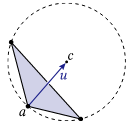
\includegraphics[width=2in]{images/auffaltung_punkteinfuegen.png}
    \caption{Illustration des Vorgehens von \citeauthor{Sharp:2019:NIT} \cite{Sharp:2019:NIT} }%\cite{shewchuk:1997:delaunay}}
    \label{fig:Punkt_einfügen}
\end{figure}
\section*{Wiederherstellung Delaunay-Eigenschaft}
Im Allgemeinen erfüllen Triangulierungen von StF-Oberflächen ebenfalls nicht die Delaunay-Eigenschaft. Laut \citet{Bobenko:2007:LaplaceBeltrami} kann die Delaunay-Eigenschaft einer jeden Triangulierung einer StF-Oberfläche durch intrinsische Kanten-Flips erhalten werden.
Ein mögliches Vorgehen einen intrinsischen Kanten-Flip Algorithmus stellt \citet{Bobenko:2006:SIGGRAPH} vor. Das Schema basiert auf dem intrinsischen LaplaceBeltrami Operator \cite{Bobenko:2007:LaplaceBeltrami}.
 \begin{figure}[H]
    \centering
    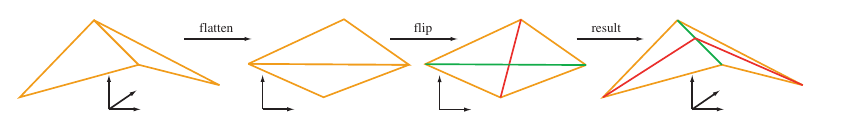
\includegraphics[width=5in]{images/intrinische_Kantenflip.png}
    \caption{Illustration des Intrinsischen Kantenflips: die beteiligten Dreiecke werden erst gemeinsam  aufgefaltet und dann die Kante geflippt.  Das Resultat ist  \textcolor{red}{die neue Kante} und \textcolor{green}{die alte Kante}  \cite{Bobenko:2006:SIGGRAPH}. }%\cite{shewchuk:1997:delaunay}}
\end{figure}
Generell gilt: Die vom intrinsischen Kanten Flip Algorithmus erzeugten Delaunay-Triangulierungmüssen nicht zwingend regulär sein, weshalb irreguläre Dreiecke im Folgen gesondert betrachtet werden müssen. 
 \begin{figure}[H]
    \centering
    \includegraphics[width=5in]{images/entstehung_irregulär.png}
    \caption{Illustration der Erzeugung von irregulären Kanten: Hier wird ein Knoten von Grad drei durch zwei intrinsische Kantenflips zu einem Knoten von Grad eins. Im Resultat sind \textcolor{red}{die neue Kante} und \textcolor{green}{die alte Kante}\cite{Bobenko:2006:SIGGRAPH}. }%\cite{shewchuk:1997:delaunay}}
\end{figure}



\section*{Winkeldefekt und irreguläre Triangulierungen}
Die bei Triangulierungen von StF-Oberflächen erlaubte intrinsische Irregularität bedeutet, dass sie Dreiecke enthalten kann, bei denen zwei Kanten identisch sind oder ein Knoten eine Kante zu sich selbst hat. Das ist ein wesentlicher Unterschied zu Triangulierungen in der euklidischen Ebene. \\

Die bei StF-Oberflächen auftretenden irregulären Kanten (beide Endknoten sind identisch) müssen daher ebenfalls gesondert betrachtet werden, denn für sie gelten die von \citet{ruppert:1995:delaunay} aufgestellten Längenlemmata nicht. Irreguläre Kanten legen sich im Allgemeinen als Schlaufe um ein Loch \citeauthor{erickson:2005:generator}, um einen Bereich mit kurzem Durchmesser oder eine Kegelspitze.\\
 \begin{figure}[H]
    \centering
    \includegraphics[width=2in]{images/irreguläre_schlaufe_loch.jpg}
    \caption{Illustration einer  irreguläre Kante $e_{v,v}$ die sich als Schlaufe um ein Loch legt }%\cite{shewchuk:1997:delaunay}}
    \label{fig:Punkt_einfügen}
\end{figure}
 


Dass sich irreguläre Kanten als Schlaufe um ein Loch oder Bereich mit kurzen Durchmesser legen, ist für die weitere Betrachtung unproblematisch, denn hier gibt es durch die Geometrie der Eingabe ein festgelegtes Minimum.  \citet{erickson:2005:generator}  schlägt in seiner Arbeit eine Methode vor, wie diese einfach berechnet werden kann.\\
Dass sich die irreguläre Kante als Schlaufe um eine Kegelspitze legt, ist für die weitere Betrachtung problematischer, denn hier kann sie sich in Richtung Kegelspitze  weiter zuziehen und somit theoretisch immer kleinere irreguläre Kanten erzeugen.
 \begin{figure}[H]
    \centering
    

\documentclass[8pt, tikz, border=5mm]{standalone}

\begin{document}

\usetikzlibrary{calc}
\usetikzlibrary{angles}
\begin{tikzpicture}




\newcommand{\radiusx}{2}
\newcommand{\radiusy}{.5}
\newcommand{\height}{4}



\coordinate (a) at (-{\radiusx*sqrt(1-(\radiusy/\height)*(\radiusy/\height))},{\radiusy*(\radiusy/\height)});

\coordinate (b) at ({\radiusx*sqrt(1-(\radiusy/\height)*(\radiusy/\height))},{\radiusy*(\radiusy/\height)});





\draw[fill=gray!30] (a)--(0,\height)--(b)--cycle;

\fill[gray!50] circle (\radiusx{} and \radiusy);

\begin{scope}
\clip ([xshift=-2mm]a) rectangle ($(b)+(1mm,-2*\radiusy)$);
\draw circle (\radiusx{} and \radiusy);

\end{scope}

\begin{scope}

\clip ([xshift=-2mm]a) rectangle ($(b)+(1mm,2*\radiusy)$);
\draw[dashed] circle (\radiusx{} and \radiusy);
\draw [ line width=0.7mm, color=blue!70](0,0.9) circle (1.5  and \radiusy);
\end{scope}

%\draw[dashed] (0,\height)|-(\radiusx,0) node[right, pos=.25]{$h$} node[above,pos=.75]{$r$};
%\draw (0,.15)-|(.15,0);


\draw  ( 0,\height) coordinate (a)  (\radiusx,0) coordinate (b) (-1* \radiusx ,0) coordinate (c); 

% \pic[draw=orange,<->,angle radius=\radiusx * 20,fill=teal!30]{angle=c--a--b};
% \draw  (0+0.5,\height-1) arc (-75:-105:2) node[above,midway]{$\Theta_{s}$};


\draw[ line width=0.7mm, color=blue!70 ](\radiusx/2,\radiusy) --  (0,\height);
\coordinate[label=below:$v$ ]  (d)   at (\radiusx/2,\radiusy) ;
\coordinate[label=above:$e_{(v,v)}$] (e)  at (0,\radiusy);
\coordinate[label=above:$e_{(v,s)}$ ] (f)  at (0,\height/2);
\coordinate[label=above:$s$] (c) at (0,\height);

\draw (\radiusx/2,\radiusy) node[]{\pgfuseplotmark{*}}; 
\draw (0,\height) node[]{\pgfuseplotmark{*}};

%\draw  ( 0, 0.8* \height) coordinate (d) node{$\Theta_s$};
\end{tikzpicture}

\end{document}
    \caption{Illustration einer  irreguläre Kante $e_{v,v}$ die sich als Schlaufe um die Kegelspitze $s$ legt \cite{erickson:2005:generator}}%\cite{shewchuk:1997:delaunay}}
    \label{fig:Punkt_einfügen}
\end{figure}
 
dass sich irreguläre Kanten als Schleife um eine Kegelspitze legen, ist wichtig, damit sich der durch den Winkeldefekt minimierte Gesamtwinkel einer Kegelspitze optimal auf den Innenwinkel eines Dreieckes verteilen kann. Da der Innenwinkel eines Dreiecks maximal $\pi$ groß sein kann, tritt dieses Phänomen nur bei Kegelspitzen mit Gesamtwinkel kleiner gleich $\pi$ auf. Daher werden wir im Folgenden besagte Kegelspitzen näher untersuchen und in Lemma \ref{le:irregulär_entfernung} zeigen, dass Kegelspitzen mit Gesamtwinkel größer $\frac{\pi}{3}$ keine Auswirkungen auf die Terminierung des Algorithmus haben. 








\section*{Größte Kreisscheibe und aufgewickelte Kanten}
Ein weiterer Unterschied ist, dass im zweidimensionalen Fall der größte Umkreisradius  einfach nach oben abgeschätzt werden kann, nämlich durch einen Kreis, der die konvexe Hülle der Triangulierung umschließt. Bei Oberflächen lässt sich diese Obergrenze nicht so leicht finden. Zudem existieren auf einer geschlossenen Oberfläche unendlich viele Möglichkeiten, zwei Knoten zu verbinden. Das hat zur Folge, dass der Algorithmus theoretisch ebenfalls immer längere Kanten erzeugen könnte, wodurch er immer neue dünne Dreiecke generieren und folglich nicht terminieren würde.\\
 \begin{figure}[H]
    \centering
    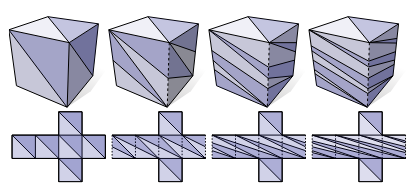
\includegraphics[width=5in]{images/aufgewickeltes_dreieck.png}
    \caption{ Illustration von aufgewickelten Kanten: die Kanten zwischen zwei festen Knoten kann theoretisch beliebig länger werden, in dem sie sich immer weiter um die geschlossene Oberfläche wickelt.\cite{Sharp:2019:NIT} }
    \label{fig:aufgewickeltung}
\end{figure}


Daher ist ebenfalls die Existenz einer möglichen Obergrenze für die Länge des Umkreisradius eines Dreiecks und seiner längsten Kante zu untersuchen. 

In Lemma \ref{le:auffaltung} zeigen wir, dass es eine natürliche Obergrenze des Umkreisradius von neu erzeugten Dreiecken gibt. Somit können auch neu erzeugte Kanten nicht unendlich lang werden, denn die längste Kante eines Dreiecks ist maximal doppelt so lange wie der Umkreisradius (siehe Abb. \ref{fig:langsteKante}).
 \begin{figure}[H]
    \centering
    \documentclass[12pt, tikz, border=5mm]{standalone}
\usepackage{tikz}
\usetikzlibrary{intersections}
\begin{document}
 \begin{tikzpicture}[thick]
% %Zeichenbereich beschneiden
% \clip(0,0)coordinate(M)circle[radius=6cm];
% %Umkreis zeichnen
% \draw[name path=k1] (M) circle [radius=5.5cm];
% %Punkt B festlegen
% \coordinate(B)at(5.5,0);
% %Konstruktion Punkt C
% \path[name path=k2](B)circle[radius=8cm];%
% \path[name intersections={of=k1 and k2,name=C}];
% %Konstruktion Punkt A
% \path[name path=g](C-2)--(B)--([turn]0:35);
% \path[name intersections={of=k1 and g,name=A}];
% % Dreieck zeichnen
% \draw(A-2)--(B)--(C-1)--cycle;
\newcommand{\radius}{2}

%Zeichenbereich beschneiden
\clip(0,0)coordinate(M)circle[radius=\radius+1];


%Umkreis zeichnen
\draw[] (M) circle [radius=\radius];


% %Punkt  festlegen
 \coordinate(B)at(\radius,0);
 \coordinate(A)at(-\radius,0);
\coordinate(C)at(0,\radius);
% %Konstruktion Punkt C
 \draw (A) -- (B) -- (C) -- cycle;
%Punkte einzeichnen und beschriften
 \foreach \p/\b/\o in {A/A/left,B/B/right,C/C/above,M/M/below}
   \node[fill=blue!80!black,circle,inner sep=1pt,label=\o:\b] at (\p){};


\end{tikzpicture}
\end{document}
    \caption{ Illustration das $d_{max}(t) \leq 2r(t)$ ist}%\cite{shewchuk:1997:delaunay}}
    \label{fig:langsteKante}
\end{figure}
 



        \chapter{Terminierung des intrinsischen Delaunay-Refinement}
\label{kap:Terminierung}

% Die Intuition des Beweises zur Terminierung beruht auf zwei Faktoren. Zum einen ist die Fläche der Triangulierung begrenzt, kann somit nicht erweitert werden. Zum anderen ist gewährleistet, dass alle Kanten, die durch den Algorithmus hinzugefügt werden, eine minimale Länge haben. Das liegt daran, dass beim Einfügen von Knoten garantiert ist,  dass keine zwei Knoten zu nahe beieinander liegen können.
% Da folglich die Kanten nicht unendlich klein werden können und die Fläche nicht größer wird, können irgendwann keine neuen Kanten mehr erzeugt werden und der Algorithmus terminiert. \\




Im Folgenden werden wir zeigen, dass der Algorithmus für eine Eingabe garantiert terminiert, für die alle Knoten $i$ einen Gesamtwinkel $\gesamtwinkel*\geq \frac{\pi}{3}$ haben und einen Winkel-Schwellenwert $\kleinsterWinkel* \leq \frac{\pi}{6}$. In der Ausgabe des Algorithmus soll für alle Innenwinkel der Triangulierung gelten, dass sie größer gleich dem gegebenen Winkel-Schwellenwert $\kleinsterWinkel*$ sind. Erst, wenn diese Bedingungen erreicht ist, terminiert der Algorithmus.


% Aus dem Kreiswinkelsatz (\ref{fig:kreiswinkelsatz}) wissen wir, dass für den kleinsten Winkel $\alpha$ eines Dreiecks 
% \begin{align*}
%     \sin(\alpha) = \frac{d}{2\cdot r}  
% \end{align*}

% gilt.

% Wird hier für  $\alpha$ die Winkeluntergrenze \kleinsterWinkel eingesetzt erhalten wir die  Obergrenze $B$ des Ur-z-kK-Verhältnisses $B = \frac{\kuezesteKante*}{2 \umkreisradius*}$.
% %TODO Satz verbessern
% Daher ist die Winkeluntergrenze \kleinsterWinkel äquivalent zu einer Obergrenze $B$ des Ur-z-kK-Verhältnisses  $\frac{\kuezesteKante*}{2 \umkreisradius*}$.\\



%Kante $d_{min}$ der Eingabe sind
% Im Folgenden zeigen wir, dass der Algorithmus \algorithmusname keine Kanten erzeugen kann, die kürzer als ein von der Eingabe Triangulierung, abhängiges Minimum $E_{min}$ ist.  Der Algorithmus kann also nur maximal so lange neue Knoten einfügen, bis alle Knoten $E_{min}$ von ihren Nachbarn entfernt sind.


Da der Beweis mit  Längenrelationen arbeitet, führen wir Hilfsfunktionen ein, um Entfernungen besser zu beschreiben. 

\subsubsection{Hilfsfunktionen}
Die Hilfsfunktionen definieren verschiedene Längen, um später im Beweis mit ihnen arbeiten zu können.
\begin{definition}
Sei $M = (V,E,T)$ eine Delaunay-Triangulierung  einer geschlossenen StF-Oberfläche, sei $t \in T$ ein Dreieck aus $M$, sei $v,u \in V$ ein Knoten aus $M$ und sei $e_{(v,u)} \in V$ eine Kante aus $M$,  dann entspricht
\begin{itemize}
    \item $d(t)$ die Länge der kürzesten Seite von $t$
    \item $d(v)$ die Länge der kürzesten zu $v$ inzidenten Kante
    \item $d(v,u)$ die Länge der Kante  $e_{(v,u)}$
    \item $r(t)$ die Länge des Umkreisradius von $t$
    \item $N(v)$ einer Liste aller zu $v$ inzident Kanten
\end{itemize}


\end{definition}



Das folgende Lemma besagt, dass für einen Iterationsschritt die jeweils neu erzeugten Kanten adjazent zum neu eingefügten Knoten sind.


%   dass für eine Kante $e$ aus der neuen Triangulierung $M^\prime$, die nicht mit dem hinzugefügten Knoten $v$ verbunden ist, bereits in der alten Triangulierung $M$ enthalten sein muss.

\begin{figure}[h!]
    \centering
    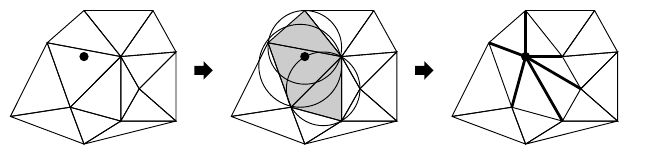
\includegraphics[width=5in]{images/adejazent.png}
    \caption{Illustration, dass alle neu erzeugten Kanten adjazent zum neu eingefügten Knoten sind \cite{shewchuk:1997:delaunay} }%\cite{shewchuk:1997:delaunay}}
    \label{fig:Punkt_einfügen}
\end{figure}
 


\begin{lemma}
\label{le:adejazent}
Sei $M = (V,E,T)$ eine intrinsische Delaunay-Triangulierung  einer geschlossenen  StF-Oberfläche und sei $M^\prime = (V^\prime,E^\prime,T^\prime)$ die Delaunay-Triangulierung  $M$ nach dem Einfügen eines neuen Knotens $v$.
 

%für jeden neu hinzugefügten Kante aus $M^\prime$, dass Sie adjazent zu $v$ ist.

%Beweis per Kontraposition: 
Wenn eine Kante $e \in E^\prime$ und $e \in N(v)$ ist und $e \in  N(v)$
%nicht Adjazent zu $v$ ,
dann folgt $e \not \in   E $.\\


% \begin{align*}
%     E^\prime \setminus E \equiv  N(v)\\
% \end{align*}


\end{lemma}

%Zeige: Ist eine Kante in der neuen Delaunay Triangulierung nicht mit dem neuen Knoten verbunden, so war sie schon in der alten Delaunay Triangulierung.


% \begin{definition}
% Eine Kante wird als Delaunay-Kante bezeichnet, wenn innerhalb der Kreisscheibe, die durch die beiden Entknoten verlauft, keine weiteren Knoten liegen.  
% \end{definition}



%Beweis per Kontraposition: wenn eine Kante $e \in E^\prime$ nicht adjazent zu $v$ ist, dann wahr sie auch in  $E$ enthalten. \\

%Angenommen es existiert in $M^\prime $ eine Kante $e \in E^\prime $  die nicht adjazent zu $v$ ist und für die gilt $e \not \in E $ 

\begin{proof}

%Beweis per Kontraposition: 
Angenommen $e \not \in  N(v)$, dann ist zu zeigen, dass $e\in E $ gilt.\\

Nach \cite[Definition 3]{Bobenko:2007:LaplaceBeltrami} ist eine Kante in einer Delaunay-Triangulierung  enthalten genau dann, wenn eine leere Kreisscheibe existiert, auf deren Rand nur ihre beiden Endknoten liegen.\\ 

    Wegen $V \subset V^\prime$  ist jede leere Kreisscheibe in $M^\prime$  auch in  $M$ enthalten. Per Annahme enthält $M$ auch beide Endknoten von $e$. Somit enthält $M$ auch $e$.     
\end{proof}


%und mindestens so lang wie ein von der Eingabe Triangulierung, abhängiges Minimum $E_{min}$ sind. 
Dünne Dreiecke sind Dreiecke mit mindestens einem Innenwinkel $\leq \frac{\pi}{6}$.  
Das nächste Lemma zeigt, dass für ein dünnes Dreieck der Umkreisradius mindestens so lang ist wie seine kürzeste Kante.


%  \citeauthor{chew:1989:guaranteed} zeigt bereits in  \cite{chew:1989:guaranteed,chew:1993:guaranteed}
%   für $\theta_{min} \leq 30^\circ$, dass sein Algorithmus terminiert.\\
%   das nächste Lemma zeigt, dass für ein als schlecht klassifizierten Dreiecke $t$ mit mindestens einem Innenwinkel kleiner $\theta_{min}$ ein  Ur-z-kK Verhältnisses größer gleich $1$ hat, in dem gilt, dass $ d(t) \leq r(t) $. 
   
% \begin{definition}
% Sei $B \geq 1 $ die Obergrenze des Ur-z-kK-Verhältnisses, so gilt jedes Dreieck mit einem Ur-z-kK Verhältnis größer $B$ als schlecht Dreieck.
% \end{definition}



% Sei B die Obergrenze dieser Metrik so gilt jedes Dreick mit einem Ur-z-kK Verhältnis grö-
% ßer als B als schlecht Dreieck. Delanuny Refinement Algorithmen könne diesen Wert nur
% verbessern und terminieren, wenn Sie für jedes Dreieck ein Wert kleiner B erzielt haben.

\begin{lemma}
\label{le:dünnes_dreieck}
Sei $t$ ein Dreieck mit kleinstem Winkel $\alpha \leq \frac{\pi}{6}$.\\
Dann gilt: 
 
 \begin{align*}
     r(t) \geq d(t).
 \end{align*} 
 \end{lemma}

\begin{figure}[h]
    \centering
    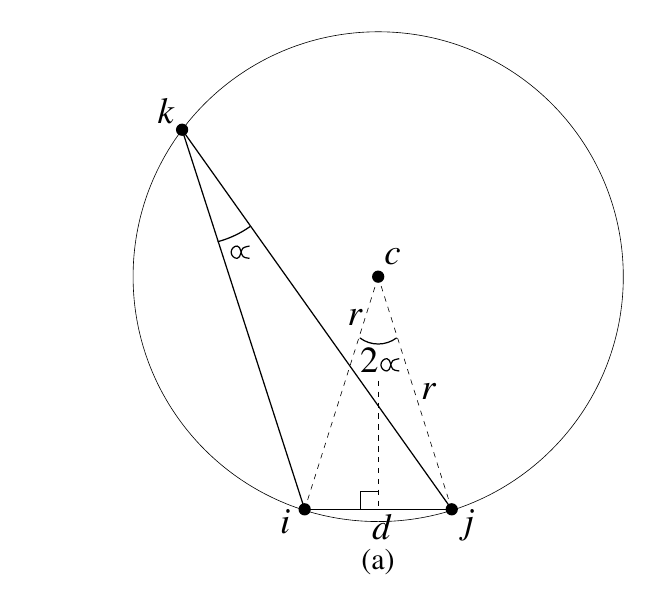
\includegraphics[width=3in]{images/Kreiswinkelsatz.png}
    \caption{Illustration des Kreiswinkelsatzes \cite{shewchuk:1997:delaunay}}
    \label{fig:kreiswinkelsatz}
\end{figure}


\newpage
\begin{proof}
Mithilfe des Kreiswinkelsatzes (\ref{fig:kreiswinkelsatz}) gilt:
\begin{align*}
d(t) &= r(t)\cdot 2\cdot\sin(\alpha)  \\
\end{align*}
Aus der Annahme $\alpha \in [0,\frac{\pi}{6}] $ folgt:

\begin{align*}
    \sin(\alpha) \leq \frac{1}{2}.
\end{align*}

Einsetzen in obige Gleichung ergibt 

\begin{align*}
     d(t) &\leq r(t).\\
\end{align*}
\end{proof}

Das nächste Lemma zeigt, dass der größte mögliche Umkreisradius bereits in der Eingabe-Triangulierung enthalten ist und durch das Einfügen neuer Punkte nur leere Kreisscheiben erzeugt werden, deren Radius kleiner gleich dem größten Radius der Eingabe ist. 



Aufgrund der Delaunay-Eigenschaft gilt jedoch, dass in der Kreisscheibe (also nicht außerhalb und nicht auf dem Rand) keine Kugelpunkte liegen. Infolgedessen ist für eingebettete leere Kreisscheiben garantiert, dass alle beteiligten Flächen sich gemeinsam und eindeutig flach in der Ebene auffalten lassen. Somit können eingebettete leere Kreisscheiben, für sich genommen, wie in der Ebene behandelt werden. 



\begin{lemma}
\label{le:auffaltung}
Sei $M = (V,E,T)$ eine intrinsische Delaunay-Triangulierung  einer geschlossenen StF-Oberfläche. Sei $K$  die größte leere Kreisscheibe auf $M$ und sei $M^\prime = (V^\prime,E^\prime,T^\prime)$ die Delaunay-Triangulierung  $M$ nach dem Einfügen eines neuen Knotens $v$. 
Dann gilt für die größte leere Kreisscheibe $K^\prime$ in $M^\prime$,

%_{i_{max},j_{max},k_{max}} mit $i_{max},j_{max},k_{max} \in V$,
\begin{align*}
    r(K) \geq r(K^\prime).\\
\end{align*}
\end{lemma}

\begin{proof}

Angenommen, durch das Einfügen von $v$ in $M$ entsteht eine neue leere Kreisscheibe $K^\prime$ mit 

\begin{align*}
    r(K^\prime) > r(K).
\end{align*}

Aus $V = V^\prime \setminus \{v\}$ und $K^\prime = \emph{}$ folgt $K^\prime \subset M$, da sie dann immer noch leer ist.\\ Das widerspricht der Annahme, dass $K$ die größte leere Kreisscheibe in $M$ ist.

\end{proof}


%  das Lemma \ref{le:dünnes_dreieck} zeigt, dass für ein $B  \geq 1$ der einfüge Radius durch eine Folge von Nachfahren eines
% Knotens nicht abnehmen Kannen. Wenn Knoten mit kleineren einfügeradien nicht erzeugt
% werden können, können keine Kanten eingeführt werden, die kürzer als die vorhandenen
% kanten sind, und die Delaunay-Verfeinerung terminiert garantiert.
% Bei der Triangulierung stückchenweise flachen-Oberfläche gibt es ein zusätzliches topologi-
% sches Besonderheit zu beachten, da sie Irregularität erlaubt, kann ein Knoten v eine Kante e
% zu sich selbst haben.




Bei Triangulierung von geschlossenen StF-Oberfläche gibt es im Vergleich zu Triangulierungen in der euklidischen Ebene zusätzliche topologische Besonderheiten zu beachten. Da sie irreguläre Dreiecke zulassen, kann ein Knoten $v$ eine Kante \irregulaereKante zu sich selbst haben.    



Die minimale Länge von regulären Kanten wird dadurch festgelegt, dass Knoten nicht zu nahe bei einander eingefügt werden können. Dies gilt nicht für irreguläre Kanten.
Dabei ist es wichtig zu unterscheiden, ob sie sich um ein Loch, einen Bereich mit kurzem Umfang oder Kegelspitze wickelt. Bei einem Loch oder einem Bereich mit kurzem Umfang existiert ebenfalls ein festes Minimum, nämlich der minimale Umfang der StF-Oberfläche. Diese lässt sich berechnen \cite{erickson:2005:generator}. Bei Kegelspitzen kann sich die Schleife  theoretisch unendlich klein zusammen ziehen. Daher müssen wir diesen fall gesondert betrachten.   



% Wir betrachten die in \cite [definition 3] {Bobenko:2007:LaplaceBeltrami}  eingeführte Definition zur Verallgemeinerung der Delauny-Triangulierung passen dabei  aber  Notation aber im Sinne der Konsistenz dieser Arbeit an.

% \begin{definition}
% Sei $M = (V,E,T)$ eine intrinsische Delaunay-Triangulation einer geschlossenen StF-Oberfläche.
% Die Delaunay-Zerlegung von $M$  ist die Vereinigung disjunkter Einheiten.
% die Delaunay-Zerlegung besteht dabei aus folgenden Mengen: Eine Teilmenge $ C \subset M$ ist eine geschlossene Einheit der Delaunay-Zerlegung, genau dann, wenn eine eingebettet leere Kreisscheibe existiert und auf ihrem Rand genau die Knoten aus $C$ liegen und zwar nur diese.
% dabei unterscheide man die Einheiten an der Anzahl ihrer Knoten: 1-Einheiten (Knoten), 2-Einheiten (Kanten) und 3-Einheiten (Dreiecksflächen)   
% \end{definition}

% Die gültige dieser Definition wurde in  \cite [Proposition 4 ff.] {Bobenko:2007:LaplaceBeltrami} gezeigt, würde an dieser Stelle aber den Rahmen dieser Arbeit sprengen.

% Es folgt unmittelbar aus der Definition: dass eine zugehöre Kante existiert, falls es eine eingebettete leere Kreisscheibe existiert, sodass die Endpunkte der Kante, und nur diese Punkte, auf dem Rand dieser Kreisscheibe liegen. Besagte Kante wird auch als Delaunay-Kante bezeichnet.



Da die Eingabetriangulierung im Allgemeinen regulär ist, können irreguläre Dreiecke erst durch das Wiederherstellen der Delaunay-Eigenschaft entstehen\cite{Bobenko:2006:SIGGRAPH,Bobenko:2007:LaplaceBeltrami}. Wir betrachten den Fall einer Schleife um eine Kegelspitze und zeigen, dass die erzeugte irreguläre Kante größer gleich der regulären Kante ist.


% nach dem Einfügen des Umkreismittelpunkts $v$ eines dünnen Dreiecks $t_{bad}$ in die Nachbarschaft einer sphärischen Kegelspitze $s$ entstehen.  
% Nun wollen wir zeigen, wann die erzeugte irreguläre Kante  \irregulaereKante von $v$ nach $v$  größer gleich der regulären Kante \regulaereKante ist.

% \begin{align*}
%     \regulaereKante* &\leq \irregulaereKante*\\
% \end{align*}


 \begin{figure}[h]
    \centering
    


\begin{tikzpicture}

\usetikzlibrary{calc}
\newcommand{\radiusx}{2}
\newcommand{\radiusy}{.5}
\newcommand{\height}{6}

  \newcommand{\delayx}{6}

\coordinate (a) at (-{\radiusx*sqrt(1-(\radiusy/\height)*(\radiusy/\height))},{\radiusy*(\radiusy/\height)});

\coordinate (b) at ({\radiusx*sqrt(1-(\radiusy/\height)*(\radiusy/\height))},{\radiusy*(\radiusy/\height)});





\draw[fill=gray!30] (a)--(0,\height)--(b)--cycle;

\fill[gray!50] circle (\radiusx{} and \radiusy);

\begin{scope}
\clip ([xshift=-2mm]a) rectangle ($(b)+(1mm,-2*\radiusy)$);
\draw circle (\radiusx{} and \radiusy);
\end{scope}

\begin{scope}
\clip ([xshift=-2mm]a) rectangle ($(b)+(1mm,2*\radiusy)$);
\draw[dashed] circle (\radiusx{} and \radiusy);
\end{scope}

%\draw[dashed] (0,\height)|-(\radiusx,0) node[right, pos=.25]{$h$} node[above,pos=.75]{$r$};
%\draw (0,.15)-|(.15,0);


\draw  ( 0,\height) coordinate (a)  (\radiusx,0) coordinate (b) (-1* \radiusx ,0) coordinate (c); 

% \pic[draw=orange,<->,angle radius=\radiusx * 20,fill=teal!30]{angle=c--a--b};
\draw  (0+0.5,\height-1.5) arc (-75:-105:2) node[above,midway]{$\Theta_{s}$};


\draw[->](\radiusx/2,-\radiusy)--node[above,rotate=100] {$e_{(v,v)}$} (0,\height);
\coordinate[label=below:$v$] (d)  at (\radiusx/2,-\radiusy);
\coordinate[label=below:$e_{(v,v)}$] (d)  at (0,-\radiusy);
\coordinate[label=above:$s$] (c) at (0,\height);


\draw[fill=gray!30]   (0+\delayx,0) coordinate[label=below:$v$] (a) -- node[above,rotate=50] {$e_{(v,s)}$} 
        (3+\delayx,6) coordinate[label=above:$s$] (b) -- node[above,rotate=-50] {$e_{(v,s)}$}
        (6+\delayx,0) coordinate[label=below:$v$] (c) --node[above] {$e_{(v,v)}$}  cycle;
        
    \draw[fill=gray!50]  ({3+\delayx+.5},{6-1}) arc (-60:-120:1) node[above,midway]{$\Theta_{s}$};
    




\end{tikzpicture}


    \caption{Illustration der Auffaltung eines irregulären Dreiecks in der euklidischen Ebene  }%\cite{shewchuk:1997:delaunay}}
    \label{fig.irreglaere}
\end{figure}

\begin{lemma}
\label{le:irregulär_entfernung}
Sei $M = (V,E,T)$ eine intrinsische Delaunay-Triangulierung  einer geschlossenen  StF-Oberfläche und  $t \in T$ ein irreguläres Dreieck aus $M$. 

%Sei $v \in t$ der zuletzt eingefügt Knoten im Dreieck $t$  und $s \in t$ eine sphärische Kegelspitze mit einem Gesamtwinkel $\gesamtwinkel*[s] \in [0,180^\circ] $. Weiterhin beschreibt \irregulaereKante die irreguläre Kante $(v,v)\in E$.\\  

Seien $v,s \in V$ die Knoten von t, \irregulaereKante die irreguläre Kante und Kegelwinkel \gesamtwinkel[s] von s gilt $\gesamtwinkel*[s] \in [\frac{\pi}{3}, \pi]$

%Wenn für alle  $v \in V$:  $\gesamtwinkel*[v] \geq 60^\circ$ gilt,
Dann folgt:
%wenn  alle Kegelspitzen in $M$ mit einem Gesamtwinkel, $\gesamtwinkel* \leq 60^\circ $ besitzt, dann gilt 
\begin{align*}
    d(\irregulaereKante*) \geq d(\regulaereKante*).\\
\end{align*}  

\end{lemma}

\begin{proof}

% laut \ref{le:regulär_entfernung} wissen wir
% Nehmen wir an, dass die regulären Kanten $e_{(s,v)}$ und $e_{(v,s)}$ zwischen $s$ und $v$ sind, größer gleich  $r_{t}$.


Aus dem Kosinussatz folgt 
\begin{align*}
    d(\irregulaereKante*^2) &=  d(e_{(s,v)})^2 + d(e_{(v,s)})^2-2 \cdot d(e_{(s,v)})  \cdot d(e_{(v,s)}) \cdot \cos(\gesamtwinkel*[s]). \\
\end{align*}

Da $d(e_{(s,v)}) = d(e_{(v,s)})$ gilt, erhalten wir durch Umformung

\begin{align*}
    % d(\irregulaereKante*)^2 &=   2\cdot d(\regulaereKante*)^2 - 2\cdot d(\regulaereKante*)^2 \cdot \cos(\gesamtwinkel*[s]) \Leftrightarrow\\ 
    % \d(\irregulaereKante*)^2 &= 2\cdot d(\regulaereKante*)^2 \cdot (1- \cos(\gesamtwinkel*[s]))\Leftrightarrow\\
    d(\irregulaereKante*)&= \sqrt{2 (1-\cos(\gesamtwinkel*[s]))}\cdot d(\regulaereKante*).\\
\end{align*}

% Nun setzten wir $\sqrt{2 (1-\cos(\gesamtwinkel*))}\cdot d(\regulaereKante*)$ für  $d(\irregulaereKante$ ein 
% \begin{align*}
%  \sqrt{2 (1-\cos(\gesamtwinkel*))}\cdot d(\regulaereKante*) \geq d(\regulaereKante*).\\   
% \end{align*}
wegen $\gesamtwinkel*[s] \in  [\frac{\pi}{3}, \pi]$, also $-1 \leq \cos(\gesamtwinkel*[s]) \leq \frac{1}{2}$  folgt
%Damit die Abschätzung gilt, muss 

\begin{align*}
     \sqrt{2 (1-\cos(\gesamtwinkel*[s]))} \geq \sqrt{2 (1-\frac{1}{2})} \geq 1\\
\end{align*}

und damit $\irregulaereKante* \geq \regulaereKante* $. 


\end{proof}


%  Lemma \ref{le:irregulär_entfernung} zeigt also, dass \algorithmusname nur irreguläre Triangulationen erzeugt, in denen die irregulären Kanten mindestens so lang sind wie die regulären Kanten des Dreiecks.\\  

Das folgende Lemma zeigt, dass durch den Algorithmus erzeugte reguläre Kanten nicht kleiner als der entsprechende Umkreisradius $r(t_{bad})$ des dünnen Dreiecks $t_{bad}$ sein können, aus dem sie erzeugt wurden.

\newpage
\begin{lemma}
\label{le:regulär_entfernung}
Sei $M = (V,E,T)$ eine Delaunay-Triangulierung  einer geschlossenen StF-Oberfläche, sei $t \in T$ ein Dreieck aus $M$, sei $v$ der Umkreismittelpunkt von $t$.   \\

 

%für alle Knoten $u\in V$ das sie mindestens $r_t$ von v entfernt sind. 


Nach dem Einfügen von $v$ in $M$ und der Wiederherstellung der Delaunay-Eigenschaft gilt für jede neu erzeugte reguläre Kante $e$, dass sie adjazent zu $v$ ist, und dass 
\begin{align*}
    d(e) \geq r(t) 
\end{align*} gilt.
%$\forall e.e\in N(v) $
\end{lemma}
 \begin{figure}[h]
    \centering
    \includegraphics[width=3in]{images/regulär_entfernung.png}
    \caption{Illustration, dass durch die Delaunay-Eigenschaft gewährleistet wird, dass neu eingefügte Knoten nicht zu nahe an bestehen Knoten liegen    \cite{SHEWCHUK:2002:chuws}}
    \label{fig:regulär_entfernung}
\end{figure}

\begin{proof}
Da $M$ die Delaunay-Eigenschaft besitzt, gilt für alle Dreiecke $t\in T$ die Delaunay-Eigenschaft, die besagt, dass im Umkreis von $t$ keine Knoten liegen, die nicht zu $t$ gehören. Nach dem Einfügen von $v$ in $M$ und dem Wiederherstellen der Delaunay-Eigenschaft gilt also für alle neu hinzugefügten regulären Kanten, dass sie inzident zu $v$ (\ref{le:adejazent}) und somit mindestens $r(t)$ lang sind.
\end{proof}

% \begin{remark}
% Eine Triangulation wird als regulär bezeichnet, wenn jedes Dreieck aus drei  Kanten und drei Knoten besteht, die jeweils paarweise verschieden sind.
% \end{remark}

% \begin{remark}
% Ein Dreieck gilt als schlecht, wenn es mindestens einen Innenwinkel $\innenwinkel* \leq 30^\circ $ besitzt.
% \end{remark} 
\newpage
Der folgende Beweis vereint nun die in den Lemmata aufgestellten Längenrelationen und zeigt, dass der Algorithmus nur Kanten erzeugen kann, die eine durch die Eingabe bestimmte Mindestlänge haben.

\begin{lemma}
\label{lem:Obergrenze}
Sei $M = (V,E,T)$ eine Delaunay-Triangulierung   einer geschlossenen StF-Oberfläche, sei $d_{min}$ die kürzeste Distanz zwischen zwei Knoten von $M$, sei $g_{min}$ der kürzeste Umfang von $M$ und sei $K_{max}$ die größte leere Kreisscheibe von $M$.

Angenommen, $M$ hat keine Kegelspitze $s$ mit einem Gesamtwinkel $\gesamtwinkel*[s] \leq \frac{\pi}{3}$. 

dann  existiert ein 
\begin{align*}
    \kappa^* = \frac{\min(d_{min}, g_{min} )}{r(K_{max)}}
\end{align*}
mit 
\begin{align*}
 \kappa^* \leq \kappa   
\end{align*}
für alle Dreiecke aus $M$.




\end{lemma}



\begin{proof}

Laut Lemma \ref{le:auffaltung} kann der Algorithmus keine Umkreisradien größer $r(k_{max})$ erzeugen.

Nehmen wir an, dass der Algorithmus \algorithmusname eine Kante, die kürzer als $\min(d_{min}, g_{min} )$ ist, einfügt. Sei \regulaereKante[(v,u)] die erste Kante dieser Art. Nach Lemma \ref{le:adejazent} ist \regulaereKante[(v,u)] inzident zum zuletzt eingefügten knoten. Sei dieser $v$ und $t_{bad}$ das zugehörige dünne Dreieck. \\

Da vor dem Einfügen von $v$ keine Kante kürzer als $\min(d_{min}, g_{min} )$ existiert hat, gilt  
\begin{align*}
    d(t_{bad}) \geq d_{min}.\\
\end{align*} 

Gemäß Lemma \ref{le:irregulär_entfernung} und \ref{le:regulär_entfernung} gilt, wenn \regulaereKante[(v,u)] eine reguläre Kante oder eine irreguläre Kante um eine Kegelspitze ist, die Abschätzung

\begin{align*}
    d(\regulaereKante*[(v,u)]) \geq r(t_{bad}).\\
\end{align*} 


Da $t_{bad}$ dünn ist, gilt nach Lemma \ref{le:dünnes_dreieck} 
\begin{align*}
    r(t_{bad}) \geq d(t_{bad}).
\end{align*}


 Daraus folgt  
 \begin{align*}
     d(\regulaereKante*[(v,u)]) \geq d_{min}.
 \end{align*}

Weiterhin gilt, wenn \regulaereKante[(v,u)] eine Schleife um einen Bereich mit kurzem Umfang oder ein Loch ist, nach Definition

\begin{align*}
     d(\regulaereKante*[(v,u)]) \geq g_{min}.
 \end{align*}



Das steht jedoch im Widerspruch zu der Annahme, dass \regulaereKante[(v,u)] kürzer ist als $\min(d_{min}, g_{min} )$. Es folgt also, dass keine eingefügte Kante kürzer ist als $\min(d_{min}, g_{min} )$. Somit kann der Algorithmus keine Dreiecke erzeugen mit \\
 \begin{align*}
    \kappa^* = \frac{ \min(d_{min}, g_{min} )}{r(k_{max})} \leq \kappa.
 \end{align*}

\end{proof}

In Lemma \ref{lem:Obergrenze} haben wir gezeigt, dass der Algorithmus nur Dreiecke erzeugt mit $\kappa \geq \kappa* $.

Nun wollen wir zeigen, dass \algorithmusname aufgrund der begrenzten Fläche terminiert. Da die Fläche der Eingabetriangulierung endlich ist, der Algorithmus in jeder Iteration neue Dreiecke erzeugt und diese Dreiecke wiederum eine Mindestfläche $A_{min}$ haben, folgt, dass der Algorithmus terminieren muss, sobald er die zur Verfügung stehende Gesamtfläche nicht mehr weiter aufteilen kann.\\  



\begin{theorem}
Sei $M = (V,E,T)$ eine Triangulierung einer geschlossenen StF-Oberfläche.
Angenommen, $M$ hat keine Kegelspitze $s$ mit einem Gesamtwinkel $\gesamtwinkel*[s] \leq \frac{\pi}{3}$ und sei  $\kleinsterWinkel* \leq \frac{\pi}{6}$ ein Winkel-Schwellenwert. 


Das intrinsische Delaunay-Refinement mit $M$ und \kleinsterWinkel als Eingabe terminiert.
\end{theorem}


% \begin{proof}
% Sei $t$ ein Dreieck aus $M$ mit einem Verhältnis von Umkreisradius zu kürzester Kante \UrzkK, Flächeninhalt $A$ und kleinsten Winkel $\theta_{min}$.




% Laut Kreiswinkelsatz gilt 
% \begin{align*}
% \theta_{min} = \arcsin(\frac{\UrzkK*}{2}) 
% \end{align*}

% Aus dem Sinussatz folgt 
% \begin{align*}
%     A \geq \frac{1}{2} \sin(\theta_{min}) \cdot d(t)^2
% \end{align*}

% Nach Lemma \ref{lem:Obergrenze} ist 
% \begin{align*}
%     \kappa \geq \kappa^* 
% \end{align*}

% Daraus folgt, dass auch eine untere Grenze für $A$ existiert und somit jedes neu erzeugte Dreieck eine Mindestfläche hat.
% \end{proof}

\begin{proof}
das lemma \ref{lem:Obergrenze} zeigt, dass es keine Kante kürzer ist als  \begin{align*}
    D = \min(d_{min},g_{min})
\end{align*}

und eine Untergrenze \begin{align*}
    \kappa^* \leq \frac{\min(d_{min},g_{min})}{r(k_{max})}
\end{align*}

von $\kappa$ existiert.

Aus dem Kreiswinkelsatz folgt, es existiert ebenfalls eine Winkeluntergrenze 

\begin{align*}
    A = \sin(\frac{\kappa^*}{2})
\end{align*}
für jedes Dreieck.\\
Aus dem Sinussatz folgt, dass jedes Dreieck eine Mindestfläche von \begin{align*}
    \frac{1}{2} \cdot \sin(A)D^2 
\end{align*}
hat.\\

Insgesamt ist die Fläche der Eingabetriangulierung begrenzt und jedes Dreieck hat eine Mindestfläche. Der Algorithmus erzeugt in jedem Schritt neue Dreiecke und da der Algorithmus nur Dreiecke mit endlich kleine Flächen erzeugen kann, muss er schließlich terminieren
\end{proof}









        
\chapter{Abschließende Beurteilung}
\section*{Fazit}
 
In der vorliegenden Arbeit wurde gezeigt, dass das intrinsische Delaunay-Refinement für Eingaben mit Winkeldefekt kleiner als $\frac{5}{3}\pi$ terminiert.
Diese Nebenbedingung ist äquivalent zu der Bedingung, dass der Winkel zwischen zwei Segmenten (feste Kanten) größer als $\frac{\pi}{3}$ ist, die von  \citeauthor{SHEWCHUK:2002:chuws} und \citeauthor{ruppert:1995:delaunay} an die Eingabe Triangulierung des Delaunay-Refinements gestellt wird. 

 %\todo[Eingabetriangulierung zusammen oder getrennt?]
 
%\textcolor{red}{genaue Zahlen und Quellen ggf. streichen, wenn kein Experiment Kapitel}
Die Auswertung einer Stichprobe des ABC-Datensatzes \cite{Koch_2019_CVPR} an 100.000 dreidimensionalen Objekten zeigte, dass die obere Schranke von  $\frac{5}{3}\pi$ in der Praxis kaum zu Komplikation führt.  Nur etwas weniger als einen Prozent der geprüften Objekte wiesen einen Winkeldefekt über der Schranke auf.

Die durchgeführten Experimente lassen darüber hinaus vermuten, dass die eigentliche Obergrenze bei $ 2 \pi -  \kleinsterWinkel*$ liegt könnte.


\section*{Ausblick}
Leider bestehen noch folgende Lücken in der Betrachtung des Winkeldefekts und des intrinsischen Delaunay-Refinements und zwar

\begin{itemize}
    \item die  Einschränkung des Winkeldefekts auf $ 2 \pi -  \kleinsterWinkel*$,
    \item Umgang mit Segmenten
    \item und Größen- und Abstufungs-Optimalität.
\end{itemize} 

 Hier gibt es noch Möglichkeiten für weiterführende Forschung.



\subsubsection{Einschränkung Gesamtwinkel}
In dieser Arbeit haben wir uns auf geschlossene Triangulierungen, welche nur Knoten enthalten, mit einem Winkeldefekt kleiner als $ \frac{5}{3}\pi$, beschränkt. Vermutlich lässt sich diese Winkeldefektbedingung auf  einen Winkeldefekt kleiner als $2\pi - \kleinsterWinkel*$ erweitern. 
%Denn der Algorithmus könnte dann zwar theoretisch Dreiecke mit einer kürzeren Kante erzeugen, dieses Dreieck würde aber nicht weiter als schlecht eingestuft, wodurch der Algorithmus ebenfalls terminiert würde. 
Die Ergebnisse einer Versuchsreihe mit den im  ABC-Datensatzes gefunden Elementen  mit einem Winkeldefekt größer als $\frac{5}{3}\pi$   unterstreichen diese Behauptung.
 

%Im Algorithmus von \citeauthor{Sharp:2019:NIT} werden dünne Dreiecke ignoriert, die an ein Dreieck mit irregulärer Kante grenzen. Dadurch terminiert sein Algorithmus ebenfalls sicher für Triangulationen mit Gesamtwinkel kleiner  $\frac{\pi}{3}$ . 

\subsubsection{Segmentbehandlung, Größen- und Abstufungs-Optimatlität}
Bisher wurde in dieser Arbeit nur gezeigt, dass der Algorithmus für einen maximalen Winkelschwellenwert von  $\frac{\pi}{6}$ sicher terminiert. Lemma \ref{lem:Obergrenze} garantiert, dass nach der Terminierung alle vom Algorithmus erzeugten Kanten mindestens $\min(d_{min},g_{m})$ lang sind. Dieses Lemma garantiert jedoch lediglich, dass der Algorithmus im Worst Case nach der Terminierung eine uniformen Triangulierung erzeugt hat. Es besteht somit keine Garantie, dass die räumliche Abstufung der Dreiecke optimal ist.\\
%\citet{ruppert:1995:delaunay} bewies dazu, dass in der Ausgangstriangulierung der Radius der Kreisscheibe eines Knotens proportional zu Länge der adjazent Kante ist. Daher werden Kantenlängen durch lokale Faktoren bestimmt und Faktoren, die außerhalb der Kreisscheibe eines Knotens, liegen beeinflussen die Länge der adjazent Kanten nur wenig. Die Größe von Dreiecken variiert schnell über kurze Entfernungen, wo eine solche Variation erwünscht ist, um die Anzahl der Dreiecke im Netz zu reduzieren. Die Größe von Dreiecken kann somit schnell über eine kurze Entfernung variieren, wo diese Variation gewünscht ist, um die Anzahl der Dreiecke in der Triangulierung zu reduzieren.
In dieser Arbeit wird dies nicht mehr für das intrinsische Delaunay-Refinement gezeigt. Jedoch wird vermutet, dass mithilfe der hier aufgestellten Lemmata und Nebenbedingungen sich \citeauthor{ruppert:1995:delaunay}s Beweise einfach übertragen lässt. Ähnliches gilt für den Umgang mit Segmenten. bestärkt wird diese Vermutung durch \citet{chew:1993:guaranteed} Ergebnisse. er zeigt für seinen zweiten Algorithmus ohne Garantien für eine optimale  räumliche Abstufung, dass er bei einem Winkelschwellenwert von maximal $\frac{\pi}{6}$. terminiert.

 

         

    % Quellen
 		%\bibliographystyle{alpha}
 		\bibliography{Quellen/Literatur}
% %%%%%%%%%%%%%%%%%%%%%%%%%%%%%%%%%%%%%%%%%%%%%%%%%%%%%%%
% % Anhang
% 	\appendix
% 		\input{attachment/Anhang}
% 		\includepdf{}
		
\end{document}